%!TEX program = pdflatex
\documentclass[11pt, a4paper]{article}

% ─── Packages ────────────────────────────────────────────────────────────────
\usepackage[T1]{fontenc}
\usepackage[utf8]{inputenc}
\usepackage{lmodern}
\usepackage[margin=2.5cm]{geometry}
\usepackage{amsmath, amssymb, bm}
\usepackage{graphicx}
\usepackage{booktabs}
\usepackage{multirow}
\usepackage{array}
\usepackage{xcolor}
\usepackage{hyperref}
\usepackage{natbib}
\usepackage{caption}
\usepackage{subcaption}
\usepackage{float}
\usepackage[section]{placeins}
\usepackage{algorithm}
\usepackage{algpseudocode}
\usepackage{enumitem}
\usepackage{parskip}
\usepackage{titlesec}
\usepackage{setspace}

\onehalfspacing
\setlength{\parindent}{0pt}
\setlength{\parskip}{6pt}

\hypersetup{
    colorlinks=true,
    linkcolor=blue!60!black,
    citecolor=green!50!black,
    urlcolor=blue!70!black
}

\graphicspath{{figures/}{../reports/exp032b/figures/}{../reports/exp032c/figures/}{../reports/exp033/figures/}{../reports/exp034/figures/}{../reports/exp035/figures/}{../reports/phase15/figures/}{../reports/phase16d/figures/}}

% ─── Title ───────────────────────────────────────────────────────────────────
\title{
    \vspace{-1cm}
    {\large Capstone Design Project --- Final Report}\\[0.8em]
    \textbf{The Effect of Reward Function Design in RL-Based\\
    BTC Grid Trading: Pareto Frontier, Winner Reversal,\\
    and OOS Robustness of Prospect-Theoretic Reward}
}

\author{
    Chanhee Lee\\
    Department of Computer Science\\
    Seoul National University of Science and Technology\\
    \texttt{happilyfly@seoultech.ac.kr}
}

\date{June 2026}

% ─── Document ────────────────────────────────────────────────────────────────
\begin{document}

\maketitle
\thispagestyle{empty}

% ─── Abstract ────────────────────────────────────────────────────────────────
\begin{abstract}
We quantitatively study the effect of \emph{reward function design} on PPO-based
reinforcement-learning policies for ATR-proportional grid trading on the BTC/USDT
1-hour market. Four reward variants---symmetric (\texttt{sym}), asymmetric
($\beta=3.42$, \texttt{asym}), Differential Sharpe Ratio
($\eta=1/28\,\mathrm{h}$, \texttt{dsr}; \citealt{moody2001dsr}), and
prospect-theoretic ($\alpha=0.68$, $\lambda=3.30$, \texttt{pt};
\citealt{kahneman1979prospect})---are each trained with 10 seeds $\times$ 1M steps
and evaluated on three environments: (i) single-split validation
(Val 2021--2023), (ii) 6-fold combinatorial purged cross-validation
\citep{lopezdeprado2018advances} 15 paths, and (iii) the unsealed
out-of-sample Test set (2024--2026, BTC \$42K\,$\to$\,\$75K bull regime).

We report four key findings.
\textbf{(1)} All four variants exceed the ATR baseline ($1.378$) by
$+21$--$36\%$ on Val, yet partition into two clusters
\{\texttt{sym}, \texttt{dsr}\} (aggressive) vs.\
\{\texttt{asym}, \texttt{pt}\} (conservative); within-cluster Cohen's $|d|<0.3$
versus across-cluster $|d|>0.8$.
\textbf{(2)} Mechanism: reward loss asymmetry directly determines trade frequency
and holding time (policy distance ratio 2.22$\times$), and the sliding-window
memory structure of DSR results in 2--6$\times$ higher hold rate than other
variants.
\textbf{(3)} Winner reverses across evaluation environments: Val=\texttt{sym}(1.87)
$\to$ CPCV=\texttt{dsr}(1.41, $p<10^{-9}$) $\to$ Test=\texttt{pt}(0.34--0.37,
consistent across two model sources, $p<0.002$).
\textbf{(4)} The OOS robustness of \texttt{pt} arises from a short-holding
mechanism: loss aversion $\lambda=3.30$ combined with concave gain $\alpha=0.68$
trains policies to exit within mean 1.4\,h (max 6\,h), thereby avoiding the
sell-side timing risk of the unseen bull regime. In contrast, \texttt{dsr} learns
long holding (mean 4.58\,h, max 169\,h = 7 days) and records the worst OOS
performance---demonstrating that the same reward formulation simultaneously
drives in-sample advantage and OOS failure.
The Val--Test distribution shift is highly significant
(KS $p<10^{-10}$, $-27\%$ variance), while policies' actions remain nearly
invariant between Val and Test ($\Delta \leq 5\%$). That is, the policies
output the same actions, but those actions produce different outcomes in the
different market regimes (Val = range-bound vs. Test = bull); the OOS
performance difference is driven by the market distribution shift, not by
policy change.

Our contribution is twofold. First, we demonstrate quantitatively that reward
design exerts its effect through a \emph{trade-off dimension in risk profile}
rather than a single Sharpe ``alpha source.'' Second, we provide quantitative
evidence that Kahneman-Tversky prospect theory confers OOS safety on
RL trading policies. Code and data:
\url{https://github.com/cosmicpotato2047/capstone-rl-trading}.
\end{abstract}

\vspace{1em}
\noindent\textbf{Keywords:} Reinforcement Learning, Grid Trading, PPO,
Reward Design, Prospect Theory, Differential Sharpe Ratio,
Combinatorial Purged CV, Out-of-Sample Generalization, Cryptocurrency

\newpage
\tableofcontents
\newpage

% ─── 1. Introduction ─────────────────────────────────────────────────────────
\section{Introduction}
\label{sec:intro}

Cryptocurrency markets exhibit micro-oscillations in hourly price that are
largely orthogonal to long-term trends, motivating \emph{grid trading} strategies
that harvest revenue from volatility itself rather than from directional
prediction. Grid trading is a simplified form of market making
\citep{avellaneda2008market}, ranging from fixed-grid rules to volatility-adaptive
variants that scale grid width by the Average True Range (ATR)
\citep{wilder1978atr}. This work studies the latter: an ATR-proportional grid
system whose grid width and limit-order placement are determined by a
reinforcement-learning policy.

\subsection{Motivation and Research Question}
\label{sec:intro_motivation}

An earlier phase of this project hypothesized that PPO RL would discover dynamic
volatility adaptation and outperform a fixed-grid baseline. Post-hoc behavioral
analysis, however, revealed that the trained policy converged to a near-constant
action $[1.0, 0.0]$ (\S\ref{sec:phase1_negative}), and that the
Bayesian-optimized ATR coefficient itself was the principal source of
performance. This negative finding suggested that the symmetric-reward $+$
ATR-proportional combination structurally absorbs the policy's degrees of
freedom, motivating the new research question of this paper:

\begin{quote}
\textbf{In BTC grid trading, how does the design of the reward function affect
the behavioral pattern and generalization performance of RL policies? In
particular, do loss-asymmetric (asymmetric, prospect-theoretic) or
risk-adjusted-return (DSR) reward formulations yield meaningful differences in
single-metric advantage or out-of-sample robustness?}
\end{quote}

\subsection{Contributions}
\label{sec:intro_contribution}

This work makes the following four contributions.

\begin{enumerate}[leftmargin=*]
\item \textbf{A statistically rigorous comparison framework for reward variants.}
Four reward functions (\texttt{sym}, \texttt{asym}, \texttt{dsr}, \texttt{pt}) are
trained in an identical environment with 10 seeds $\times$ 1M steps, and pairwise
statistical tests (Cohen's $d$, bootstrap P(A$>$B), IQM, 5\% CVaR) are applied
following \citet{henderson2018rlreproducibility}'s reproducibility guidelines.
\item \textbf{Pareto-frontier discovery (multi-dimensional trade-off).}
Rather than a single ``best variant'' winner, the four variants statistically
partition into two clusters \{\texttt{sym}, \texttt{dsr}\} vs.\
\{\texttt{asym}, \texttt{pt}\} forming a Pareto-like frontier on the
Sharpe--MDD plane (\S\ref{sec:pareto}). This outcome falls into none of the
pre-registered scenario branches (A optimistic / B neutral / C pessimistic),
so we name it \emph{Scenario D} and formalize it in
\S\ref{sec:pareto_scenario_d}.
\item \textbf{Causal chain: reward $\to$ behavior $\to$ outcome.} Policy-level
differences across variants are quantified on 1.04M step trajectories via a
policy-distance matrix (within-cluster 0.129 vs.\ across-cluster 0.286), regime-
specific trade/hold statistics, and action distribution comparison, confirming
the mechanism reward loss asymmetry $\to$ reduced trade frequency $\to$
conservative cluster (\S\ref{sec:mechanism}).
\item \textbf{Winner reversal across evaluation environments and OOS robustness
of prospect theory.} The winner reverses completely across single-split Val
(\texttt{sym} 1\textsuperscript{st}) $\to$ CPCV multi-split
(\texttt{dsr} 1\textsuperscript{st}) $\to$ the unsealed Test
(\texttt{pt} 1\textsuperscript{st}, consistent across two sources $p<0.002$)
(\S\ref{sec:robustness}). Trajectory analysis attributes \texttt{pt}'s OOS
robustness to its loss aversion ($\lambda=3.30$) and concave utility
($\alpha=0.68$), which train policies to exit within an average of $1.4$\,h
and thereby avoid sell-side timing risk in the unseen bull regime. This
provides quantitative evidence that the Kahneman--Tversky prospect theory
\citep{kahneman1979prospect} confers OOS safety on RL trading policies.
\end{enumerate}

\subsection{Paper Structure}
\label{sec:intro_structure}

Section \ref{sec:related} surveys related work on RL trading, reward design
theory, and evaluation methodology. Section \ref{sec:method} details the
environment design (MDP, ATR formula, four reward variants) and PPO training.
Section \ref{sec:phase1_negative} briefly reproduces the Phase 1 negative
finding (``RL $=$ Fixed $[1.0, 0.0]$'') as motivation. Section \ref{sec:pareto}
reports the two-cluster Pareto-frontier result on Val (Scenario D), while
Section \ref{sec:mechanism} quantifies the mechanism. Section
\ref{sec:robustness} presents the robustness trio: slippage
(\S\ref{sec:slippage}), CPCV multi-split (\S\ref{sec:cpcv}), and the central
contribution of this paper---the Test OOS evaluation and the mechanistic basis
of prospect theory's robustness (\S\ref{sec:oos}). Section \ref{sec:discussion}
discusses distribution shift quantification and limitations, and Section
\ref{sec:conclusion} concludes.

% ─── 2. Related Work ─────────────────────────────────────────────────────────
\section{Related Work}
\label{sec:related}

This paper lies at the intersection of four areas: (i) market making and grid
trading, (ii) reinforcement-learning-based trading, (iii) reward-design theory,
and (iv) evaluation methodology for trading policies. This section surveys the
key prior work in each area and clarifies where our contribution lies.

\subsection{Market Making and Grid Trading}
\label{sec:related_grid}

The academic ancestor of grid trading is the market-making model of
\citet{avellaneda2008market}. Their analysis derives a closed-form optimal
policy for a risk-averse market maker who faces inventory risk and must place
\emph{asymmetric} bid/ask quotes around the mid-price. Two key insights are
that (a) the bid--ask spread is a function of volatility and remaining time
horizon, and (b) inventory skew shifts the quote midpoint asymmetrically. Grid
trading is a simplified practical variant of this model in which orders are
placed on a pre-defined ladder of price levels in order to monetize
micro-volatility.

The standard mechanism for adapting grid widths to market volatility is the
Average True Range \citep{wilder1978atr} (ATR; 14-period moving average is the
default). ATR is a smoothed average of the true price range and provides a
simple, robust rule that automatically widens the grid in volatility-cluster
regimes. ATR-proportional grids of the form $\Delta = c \cdot \mathrm{ATR}$
(with proportional coefficient $c$) are widely used in practice and serve as
the baseline of this paper.

Most prior academic work in this area is limited to the analysis of
\emph{rule-based} policies, with relatively few attempts to learn the grid-width
decision from data. This paper adopts a structure in which the proportional
coefficient and the number of grid splits in the ATR formula are dynamically
determined by an RL policy, while quantitatively analyzing how the design of
the reward function influences the resulting learned policy's behavior.

\subsection{Reinforcement Learning for Trading}
\label{sec:related_drl}

The standard DRL baseline for cryptocurrency trading is the PPO/A2C/DQN
comparison framework of \citet{zhang2020drl}, which feeds price time series
directly into a PPO policy and shows consistent improvements over simple
buy-and-hold (B\&H) and moving-average crossover strategies. The ACM survey of
\citet{sun2023rl} and the more recent review of \citet{liu2025review} both
identify two open problems in the area: \emph{(a) interpretability of policy
behavior and (b) generalization across market regimes}. This paper addresses
both directly: \S\ref{sec:mechanism} quantifies the causal chain from reward
form to behavioral difference, and \S\ref{sec:robustness} documents
out-of-sample (OOS) generalization phenomena that are not captured by
single-split validation alone.

Four prior works are directly relevant. \citet{liu2021bitcoin} feed the
output of an LSTM price predictor into the state of a PPO trading policy in a
two-stage pipeline. The limitation of this approach is that prediction errors
propagate directly into trading decisions; this paper bypasses the limitation
by \emph{eliminating} the price-prediction stage and using a volatility-adaptive
grid structure instead. \citet{yasin2024rl} compare DQN/PPO/A2C with 20
technical indicators, but their action space is discrete buy/sell with no hold
action. This paper adopts a continuous two-dimensional action (aggressiveness
and profit target) that supports fine-grained grid control.
\citet{pham2025dqn} use DQN to select one of five predefined strategies as a
meta-strategy, but the strategies themselves are not learned.
\citet{bandarupalli2025risk} augment PPO with a volatility penalty and a
transaction-cost term, but stay at the level of hyperparameter tuning within
a single reward variant and do not compare across reward \emph{forms}, which
is the focus of this paper.

A particularly relevant prior work is \citet{gort2022backtest}, who
empirically show that \emph{single-split train/test results do not guarantee
OOS generalization} in cryptocurrency DRL trading, and recommend CPCV
(Combinatorial Purged Cross-Validation) and DSR (Deflated Sharpe Ratio). This
paper adopts those recommendations, using Val (2021--2023), CPCV (6-fold inside
the Train partition), and Test (2024-- unsealed) environments concurrently.
Our \emph{winner reversal} finding (Val \texttt{sym} $\to$ CPCV \texttt{dsr}
$\to$ Test \texttt{pt}) is a quantitative confirmation that Gort et al.'s
concern reappears in the dimension of reward-variant selection.

In summary, whereas prior DRL trading literature focuses
on comparing algorithms and state designs under a \emph{single} reward function,
this paper performs a controlled comparison of \emph{four reward functions} on
top of the same algorithm (PPO) and the same environment, and separately
measures their effects on in-sample / multi-split / OOS environments.

\subsection{Reward-Design Theory}
\label{sec:related_reward}

The four reward variants compared in this paper draw from three theoretical
lineages in reinforcement learning and behavioral economics. (i) Symmetric
(\texttt{sym}) is the standard PnL-return reward and serves as our baseline.
(ii) Asymmetric (\texttt{asym}) places a positive weight $\beta>1$ on losses,
a simple first-order approximation of a risk-averse utility. (iii) Differential
Sharpe Ratio (\texttt{dsr}) is the formulation of \citet{moody2001dsr}.
(iv) Prospect-theoretic reward (\texttt{pt}) directly uses the utility function
of \citet{kahneman1979prospect} and \citet{tversky1992cumulative},
$v(x) = \mathrm{sgn}(x) |x|^\alpha$ for $x \geq 0$ and $-\lambda |x|^\alpha$
for $x < 0$, as a per-step reward.

The DSR formulation of \citet{moody2001dsr} uses the \emph{differential change
of the online Sharpe-ratio estimator} as the step reward, tracking first and
second moments via exponentially-weighted moving averages (EWMA, decay rate
$\eta$). This has two implications for RL training: (a) it directly optimizes
a risk-adjusted return rather than raw PnL, and (b) the sliding-window memory
imposes a \emph{multi-step temporal dependency} on the policy. As we show in
\S\ref{sec:mechanism}, this memory structure is what causes the \texttt{dsr}
policy to learn 2--6$\times$ longer holding times than the other variants---a
property that becomes the in-sample advantage of \S\ref{sec:robustness} and
the OOS failure of \S\ref{sec:oos} — the same causal mechanism viewed
from two evaluation angles.

Prospect theory \citep{kahneman1979prospect} is a foundational model of
human decision making under risk, with two characteristic parameters:
(a) loss aversion $\lambda \approx 2.25$ (standard value from
\citealt{tversky1992cumulative}) and (b) the concavity exponent
$\alpha \approx 0.88$. While the theory has been widely used to describe
human trader behavior (e.g., the disposition effect — holding losing positions
too long while realizing gains too early), \emph{direct use of
prospect-theoretic utility as an RL reward} is rare in the literature. This paper directly implements the
\citet{kahneman1979prospect} utility as an RL reward (with $\alpha=0.68$,
$\lambda=3.30$, tuned by Optuna) and quantitatively establishes the OOS
robustness that the resulting policy exhibits.

\citet{ng1999reward}'s policy-invariance theorem of potential-based reward
shaping states that ``a monotone transformation of the reward signal does not
alter the policy learned by RL.'' At first glance, this paper's comparison of
four reward variants may appear to conflict with the theorem, but it does not:
the \texttt{sym} $\to$ \texttt{asym}/\texttt{pt} transformations are
\emph{non-potential-based} (they apply an asymmetric scale on the negative
half-line), while \texttt{dsr} is not a simple per-step reward transformation
but a \emph{state-extended} reward (the sliding-window moments effectively
become part of the state). Our reward-variant comparison thus lies outside the
scope of the Ng et al.\ theorem, and indeed we confirm in
\S\ref{sec:mechanism} that policy behavior differs across variants in a
statistically significant manner.

\subsection{Evaluation Methodology}
\label{sec:related_eval}

The two principal pitfalls in evaluating RL trading policies are (a) backtest
overfitting and (b) seed dependence of results.
\citet{henderson2018rlreproducibility} empirically demonstrate that seed
variability alone can produce large differences for the same algorithm, and
propose 5--10 seed statistical comparisons, IQM (Interquartile Mean), and
bootstrap confidence intervals as standard recommendations. This paper uses
10 seeds per variant (Val/exp033) and 100 models (Test), and applies pairwise
Cohen's $d$ and bootstrap $\mathrm{P}(A>B)$ to all comparisons.

\citet{lopezdeprado2018advances} (Ch.\ 8) proposes \emph{Combinatorial Purged
Cross-Validation} (CPCV), which avoids train/test leakage in time-series data
while leveraging $\binom{N}{k}$ split combinations to strengthen the
generalization guarantees of single-split results. We adopt 6-fold CPCV
(15 paths) in \S\ref{sec:cpcv}.

\citet{lopezdeprado2014dsr}'s \emph{Deflated Sharpe Ratio}
(DSR\textsuperscript{*}) is a statistical-significance test on the Sharpe
ratio that corrects for the number of backtest trials and for the skewness/kurtosis
of the underlying distribution. We apply Bonferroni 4-way correction together
with DSR\textsuperscript{*} testing to the multiple comparisons of CPCV
results (\S\ref{sec:cpcv}), and confirm that all four reward variants are
significant relative to the ATR baseline at $p<0.001$.

The methodological distinctiveness of this paper is the \emph{simultaneous use
of three evaluation environments} (Val / CPCV / Test) that allowed us to
discover the winner reversal. Studies relying solely on single-split or solely
on CPCV cannot expose OOS generalization failure, and studies relying solely
on OOS cannot expose the in-sample conservatism of \texttt{pt}. The
simultaneous application of three environments is, in our view, a methodological
contribution: it generalizes the multi-evaluation recommendations of
\citet{henderson2018rlreproducibility} and \citet{gort2022backtest} to the
single dimension of reward-variant comparison.

% ─── 3. Method ───────────────────────────────────────────────────────────────
\section{Method}
\label{sec:method}

\subsection{MDP Formulation}
\label{sec:mdp}

We cast single-asset dynamic grid trading on the BTC/USDT 1-hour series as a
finite-horizon Markov decision process $\mathcal{M} = (\mathcal{S},
\mathcal{A}, P, R, \gamma)$. An episode runs for 720 hours (30 days) starting
from a randomly chosen step within the training/validation range, and each
step $t$ corresponds to a 1-hour price bar.

\paragraph{State $\mathcal{S} \subset \mathbb{R}^7$.}
The observation $\mathbf{s}_t = (s_t^{(0)}, \ldots, s_t^{(6)})$ couples market
and portfolio state:

\begin{align}
s_t^{(0)} &= \log\!\left(p_t \,\big/\, \overline{p}_{t, 168}\right) &&
\text{(price vs.\ 1-week mean)} \\
s_t^{(1)} &= \frac{\bar{p}^{\mathrm{avg}}_t - p_t}{\bar{p}^{\mathrm{avg}}_t} &&
\text{(divergence from average cost)} \\
s_t^{(2)} &= \frac{h_t \cdot p_t}{C_0} &&
\text{(holdings value / capital)} \\
s_t^{(3)} &= \frac{c_t}{C_0} &&
\text{(cash ratio)} \\
s_t^{(4)} &= \frac{\mathrm{ATR}_{168}(p)}{p_t} &&
\text{(volatility)} \\
s_t^{(5)} &= \frac{p_t - p_{t-72}}{p_{t-72}} &&
\text{(short-term trend, 3d)} \\
s_t^{(6)} &= \frac{p_t - p_{t-720}}{p_{t-720}} &&
\text{(long-term trend, 30d)}
\end{align}

Here $p_t$ is the bar close, $\bar{p}^{\mathrm{avg}}_t$ is the average cost of
the current position (set to 0 when no position is held, in which case
$s_t^{(1)}$ is also 0), $h_t$ is the BTC quantity, $c_t$ the cash balance, and
$C_0 = 10{,}000$ USDT is the initial capital. $\mathrm{ATR}_{168}$ is the
Average True Range \citep{wilder1978atr} computed over a 168-bar (1-week)
window, and $\overline{p}_{t,168}$ is the corresponding simple moving average.
All components are pre-normalized by a 168-bar rolling z-score computed on the
training set and clipped to $[-5, 5]$.

\paragraph{Action $\mathcal{A} = [0,1]^2$.}
At each step the policy outputs a continuous 2D action $\mathbf{a}_t =
(a_t^{(0)}, a_t^{(1)})$. The first coordinate $a_t^{(0)}$ (\emph{aggressiveness})
controls two buy limit orders, and $a_t^{(1)}$ (\emph{profit target}) controls
two sell limit orders. We avoid a discrete buy/sell/hold action space because
fine-grained grid width adjustment and volatility adaptation are most naturally
expressed in continuous values; discretization would artificially limit the
expressiveness of the action space.

\paragraph{ATR-proportional grid formula.}
Grid widths and positions are determined through volatility-normalized action
coordinates. With $r_t = \mathrm{ATR}_{168}(p) / p_t$, current price $p_t$, and
average cost $\bar{p}^{\mathrm{avg}}_t$,
\begin{align}
g^{\mathrm{buy\_hi}}_t  &= r_t \cdot (A_b + B_b \cdot a_t^{(0)}) \\
g^{\mathrm{buy\_lo}}_t  &= r_t \cdot (C_b + D_b \cdot a_t^{(0)}) \\
g^{\mathrm{sell\_mkt}}_t &= r_t \cdot (A_s + B_s \cdot a_t^{(1)}) \\
g^{\mathrm{sell\_cost}}_t &= r_t \cdot (C_s + D_s \cdot a_t^{(1)})
\end{align}
Quote prices:
\begin{equation}
q^{\mathrm{buy\_hi}}_t = p_t (1 - g^{\mathrm{buy\_hi}}_t), \quad
q^{\mathrm{buy\_lo}}_t = p_t (1 - g^{\mathrm{buy\_lo}}_t)
\end{equation}
\begin{equation}
q^{\mathrm{sell\_mkt}}_t = p_t (1 + g^{\mathrm{sell\_mkt}}_t), \quad
q^{\mathrm{sell\_cost}}_t = \bar{p}^{\mathrm{avg}}_t (1 + g^{\mathrm{sell\_cost}}_t)
\end{equation}
The coefficients $\{A_b, B_b, C_b, D_b, A_s, B_s, C_s, D_s\}$ are fixed
environment constants, with values reported in \S\ref{sec:atr_baseline}. Only
the \texttt{sell\_cost} quote is anchored at the average cost; the choice
explicitly exposes ``break-even recovery'' to the policy.

\paragraph{Reward.}
The baseline (\texttt{sym}, symmetric) form is the 1-step PnL ratio:
\begin{equation}
r_t^{\mathrm{sym}} = \frac{E_t - E_{t-1}}{C_0}, \quad
E_t = c_t + h_t \cdot p_t
\end{equation}
Transaction fees are already deducted from $c_t$ inside
\texttt{\_execute\_buy} and \texttt{\_execute\_sell}, so no separate subtraction
appears in the reward. All four reward variants in this paper are defined as
functions of $r_t^{\mathrm{sym}}$ and detailed in \S\ref{sec:reward_variants}.

\subsection{Trading-Environment Dynamics}
\label{sec:env_dynamics}

This subsection details order execution, the cycle definition, and the
transaction-cost model.

\paragraph{Limit-order execution.}
Fill decisions for the four quotes use the next bar's high/low
$(p^{\mathrm{H}}_{t+1}, p^{\mathrm{L}}_{t+1})$:
\begin{equation}
\begin{aligned}
&p^{\mathrm{L}}_{t+1} \leq q^{\mathrm{buy\_hi}}_t  \Rightarrow
\text{fill at $q^{\mathrm{buy\_hi}}_t$} \\
&p^{\mathrm{L}}_{t+1} \leq q^{\mathrm{buy\_lo}}_t  \Rightarrow
\text{fill at $q^{\mathrm{buy\_lo}}_t$} \\
&p^{\mathrm{H}}_{t+1} \geq q^{\mathrm{sell\_mkt}}_t \Rightarrow
\text{fill at $q^{\mathrm{sell\_mkt}}_t$} \\
&p^{\mathrm{H}}_{t+1} \geq q^{\mathrm{sell\_cost}}_t \Rightarrow
\text{fill at $q^{\mathrm{sell\_cost}}_t$}
\end{aligned}
\end{equation}
When both buy and sell quotes are filled in the same bar we apply a
\emph{sell-first} rule, prioritizing inventory liquidation. The fill price is
the \emph{quote price itself}, not the next-bar extreme. Filling at the
next-bar extreme injects favorable bias into the simulation; we therefore
discarded an earlier ``next\_low/next\_high'' execution rule and use only the
limit-order rule throughout this paper.

\paragraph{Cycle definition.}
A cycle starts when the \emph{first buy fills while holdings = 0} and ends
when subsequent sells return holdings to 0. Multiple partial buys/sells can
occur inside a single cycle, and the cycle return is
$\mathrm{cycle\_pnl} = (c_{\text{end}} - c_{\text{start}}) / c_{\text{start}}$.
At the start of each cycle, the slot size used for the cycle is set:
\begin{equation}
\text{slot\_size}_{\text{cycle}} =
\frac{c_{\text{start}}}{n_{\text{splits}}}, \quad
\text{order\_size} = \frac{\text{slot\_size}}{n_{\text{buy\_orders}}}
\end{equation}
We use $n_{\text{splits}}=2$ and $n_{\text{buy\_orders}}=2$ (the best values
from Phase 2 Optuna Trial \#34). \texttt{threshold\_basis} is fixed to
\texttt{avg\_price}, meaning the ``liquidate all'' detection uses the average
cost.

\paragraph{Transaction-cost model.}
Transaction costs are set to \emph{0.05\% per side} (Binance maker fee). On a
buy, the filled quantity is $\Delta h = \text{order\_size} \cdot (1 - f) / q$
and the cash change is $\Delta c = -\text{order\_size}$, so the fee is already
reflected in $c_t$. In \S\ref{sec:slippage} (exp033) we add an additional
slippage $\sigma = 0.02\%$ that modifies fill prices to
$q^{\mathrm{buy}} \cdot (1 + \sigma)$ and $q^{\mathrm{sell}} \cdot (1 - \sigma)$.
Slippage is not applied to the base environment and appears only in the
robustness analysis.

\subsection{ATR Baseline}
\label{sec:atr_baseline}

The comparison baseline \emph{shares the environment and grid formula} with
our RL policies but determines actions via a rule. Concretely, the ATR
baseline reuses the grid formulas of \S\ref{sec:mdp} for $g^{\mathrm{buy\_hi}},
g^{\mathrm{buy\_lo}}, g^{\mathrm{sell\_mkt}}, g^{\mathrm{sell\_cost}}$ with all
RL action degrees of freedom \emph{zeroed} ($a_t^{(0)} = a_t^{(1)} = 0$, so
that the $B_b, D_b, B_s, D_s$ terms drop and the grid widths are fixed
time-independent constants determined entirely by $A_b, C_b, A_s, C_s$). The
coefficient values come from Phase 2 Optuna Trial \#34:

\begin{table}[!htbp]
\centering
\caption{Grid coefficients of the ATR baseline (Phase 2, Optuna Trial \#34).}
\begin{tabular}{lcclcc}
\toprule
Coef. & Value & Role & Coef. & Value & Role \\
\midrule
$A_b$ & 1.665 & buy\_hi base width & $A_s$ & 0.285 & sell\_mkt base width \\
$C_b$ & 6.070 & buy\_lo base width & $C_s$ & 1.951 & sell\_cost base width \\
$B_b$ & 1.748 & buy\_hi action sensitivity & $B_s$ & 1.950 & sell\_mkt action sens.\ \\
$D_b$ & 18.683 & buy\_lo action sensitivity & $D_s$ & 7.500 & sell\_cost action sens.\ \\
\bottomrule
\end{tabular}
\label{tab:atr_coefs}
\end{table}

The ATR baseline yields Val Sharpe $1.378$ without slippage, dropping to
$0.835$ when slippage of $0.02\%$ is added.

\subsection{Four Reward Variants}
\label{sec:reward_variants}

We now define the four reward variants that form the principal comparison unit
of this paper. All are expressed as functions of $x_t := r_t^{\mathrm{sym}} =
(E_t - E_{t-1}) / C_0$ and differ \emph{only} in functional form; the state,
action, ATR grid, and fee model are otherwise identical.

\paragraph{(i) Symmetric (\texttt{sym}).}
\begin{equation}
r_t^{\mathrm{sym}} = x_t = \frac{E_t - E_{t-1}}{C_0}
\end{equation}
No hyperparameter. Baseline of this paper.

\paragraph{(ii) Asymmetric (\texttt{asym}).}
\begin{equation}
r_t^{\mathrm{asym}} =
\begin{cases}
x_t & \text{if } x_t \geq 0 \\
\beta \cdot x_t & \text{if } x_t < 0
\end{cases}, \quad \beta > 1
\end{equation}
A first-order approximation of a risk-averse utility, weighting losses by
$\beta$. An Optuna 30-trial $\times$ 200k-step search over the range
$[1.0, 4.0]$ to maximize Val Sharpe selected the best $\beta = 3.420$.

\paragraph{(iii) Differential Sharpe Ratio (\texttt{dsr}).}
The formulation of \citet{moody2001dsr}. Given an EWMA decay rate $\eta$,
online estimates of the first and second return moments evolve as
\begin{align}
A_t &= A_{t-1} + \eta \, (x_t - A_{t-1}) \\
B_t &= B_{t-1} + \eta \, (x_t^2 - B_{t-1}) \\
\Delta A_t &= x_t - A_{t-1}, \quad \Delta B_t = x_t^2 - B_{t-1}
\end{align}
The DSR step reward is the differential of the on-line Sharpe estimator
$\hat{S}_t = A_t / \sqrt{B_t - A_t^2}$:
\begin{equation}
r_t^{\mathrm{dsr}} =
\frac{B_{t-1} \, \Delta A_t - \tfrac{1}{2} A_{t-1} \, \Delta B_t}
     {(B_{t-1} - A_{t-1}^2)^{3/2}}
\end{equation}
A 30-trial Optuna search over $[1/720, 1/24]$ (log-uniform) selected the best
$\eta = 0.0352 \approx 1/28\,\text{h}$, an EWMA window of approximately
1.2~days.

\paragraph{(iv) Prospect-theoretic (\texttt{pt}).}
The utility function of \citet{kahneman1979prospect} and
\citet{tversky1992cumulative} applied directly as a step reward:
\begin{equation}
r_t^{\mathrm{pt}} =
\begin{cases}
\mathrm{sgn}(x_t) \, |x_t|^{\alpha} & \text{if } x_t \geq 0 \\
-\lambda \, |x_t|^{\alpha} & \text{if } x_t < 0
\end{cases}, \quad 0 < \alpha \leq 1, \quad \lambda \geq 1
\end{equation}
$\alpha < 1$ encodes the concavity of the utility (diminishing marginal
utility of gains), and $\lambda > 1$ encodes loss aversion. The standard
values from \citet{tversky1992cumulative}, fitted to human behavior, are
$\alpha = 0.88$ and $\lambda = 2.25$. The Val-Sharpe-maximizing values for our
RL policy, however, are $\alpha = 0.683$ and $\lambda = 3.303$, found by
Optuna 30 trials over $\alpha \in [0.5, 1.0]$ and $\lambda \in [1.0, 4.0]$.
The fact that RL prefers a \emph{more concave} utility and \emph{stronger
loss aversion} than the human standard is consistent with the mechanism in
\S\ref{sec:mechanism} and the OOS robustness reported in \S\ref{sec:oos}.

\paragraph{Optuna search summary.}
For each of the three variants \texttt{asym}, \texttt{dsr}, \texttt{pt} we ran
30 trials $\times$ 200k steps using a TPE sampler
\citep{akiba2019optuna} (seed=42, MedianPruner with
$n_{\text{startup}}=5$). The total training cost was $3 \times 30 \times
200\text{k} = 18$M steps, taking approximately 2 hours on a Windows 11
CPU with $n_{\text{envs}}=4$. \texttt{sym} has no hyperparameter and skips
this stage.

\subsection{PPO Training and the Stabilization Package}
\label{sec:ppo_stab}

Policy training uses PPO \citep{schulman2017ppo} from stable-baselines3
\citep{raffin2021sb3}. Standard PPO hyperparameters
($\gamma=0.99$, $\lambda_{\mathrm{GAE}}=0.95$, clip
$\epsilon=0.2$, $v_f$ coef $=0.5$, gradient clip $=0.5$, MLP policy
$[64, 64]$, batch=256, $n_{\text{epochs}}=10$, $n_{\text{steps}}=4096$,
$n_{\text{envs}}=4$) follow stable-baselines3 defaults. To mitigate the
reward sparsity of our environment (the per-step reward is near 0 when no
fill occurs) and the late-stage policy collapse observed in Phase 2
(exp020--022), we add the following \emph{stabilization package} (exp030):

\begin{enumerate}[leftmargin=*]
\item \textbf{Learning-rate linear decay}: $\alpha_t$ linearly decays from
$3 \times 10^{-4}$ to $1 \times 10^{-5}$ over training. This bounds the size
of late-stage policy updates and dampens post-best collapse.
\item \textbf{Entropy coefficient annealing}: $c_{\text{ent}}$ linearly anneals
from $0.01$ to $0.001$, ensuring sufficient initial exploration while
encouraging convergence to a near-deterministic policy late in training.
\item \textbf{Target KL early stop}: $\text{target\_kl}=0.02$ measures the KL
divergence after each minibatch update and aborts the update for that batch if
the threshold is exceeded, preventing PPO from making myopic large policy
changes.
\item \textbf{Best-model checkpoint}: Val Sharpe is evaluated every 50k steps
($n_{\text{eval\_episodes}}=5$) and the weights at the best Val Sharpe are
saved separately, providing protection against late-stage collapse.
\end{enumerate}

The package was developed in exp030 (with \texttt{sym} reward) and produced
Val Sharpe best $1.974$ at step 550k, falling to final $1.209$ at step 1M.
Because the collapse pattern after step 700k persists despite the package,
\emph{all evaluations in this paper use the best checkpoint}; the final model
is never used.

\subsection{Evaluation Protocol}
\label{sec:eval_protocol}

We use \emph{three evaluation environments concurrently}. The data partition
is strict time-order to prevent leakage:

\begin{table}[!htbp]
\centering
\caption{Data partition.}
\begin{tabular}{lll}
\toprule
Partition & Range & Bars (approx.) \\
\midrule
Train & 2017-08-17 \,--\, 2020-12-31 & $\sim$30{,}000 \\
Val (single-split) & 2021-01-01 \,--\, 2023-12-31 & $\sim$26{,}000 \\
Test (sealed) & 2024-01-01 \,--\, 2026-04 & $\sim$20{,}000 \\
\bottomrule
\end{tabular}
\label{tab:data_split}
\end{table}

\paragraph{Val (single-split).}
The main comparison environment of \S\ref{sec:pareto}. For each reward variant
we train 10 seeds $\times$ 1M steps and evaluate the best\_model on the entire
Val range with $n_{\text{eval\_episodes}}=5$, producing per-seed
Sharpe/MDD/Calmar/trade-count/return.

\paragraph{CPCV 6-fold.}
The multi-split environment of \S\ref{sec:cpcv}. Following
\citet{lopezdeprado2018advances}, we apply 6-fold Combinatorial Purged
Cross-Validation \emph{inside the Train partition}, producing
$\binom{6}{2}=15$ paths (each consisting of 5 months of training plus
1 month of evaluation). A 1-week purge gap between train and evaluation folds
prevents information leakage. We execute 4 variants $\times$ 15 paths $\times$
1 seed = 60 runs.

\paragraph{Test (unsealed).}
The OOS environment of \S\ref{sec:oos}. For academic rigor, following
\citet{gort2022backtest}, Test was \emph{kept sealed from any search or
hyperparameter decision} until exp035 (May 16, 2026). After unsealing, we
evaluate 100 RL models (4 variants $\times$ multi-seed/seed-pair) along with
the ATR baseline and Buy-and-Hold on Test.

\paragraph{Statistical tests.}
All pairwise comparisons report Cohen's $d$ and bootstrap $\mathrm{P}(A > B)$
($10^4$ resamples). Single-sided t-tests against ATR on CPCV use Bonferroni
4-way correction along with the Deflated Sharpe Ratio test of
\citet{lopezdeprado2014dsr}. To report evaluation variability and distributional
skew, we follow \citet{henderson2018rlreproducibility} and add IQM
(Interquartile Mean) and 5\% CVaR as secondary metrics.

\subsection{Pre-Registered Hypotheses}
\label{sec:hypotheses}

To prevent ex-post rationalization, this paper's experimental comparison is
guided by the following pre-registered hypotheses. H1--H4 were registered at
the start of the paper; H5 was discovered after the Test unsealing and is
therefore stated separately as a post-hoc hypothesis.

\begin{table}[!htbp]
\centering
\small
\caption{Pre-registered hypotheses H1--H4 and post-hoc hypothesis H5.}
\begin{tabular}{p{1.8cm}p{5cm}p{6.5cm}}
\toprule
Hypothesis & Name & Definition \\
\midrule
H1 & sym RL $\approx$ ATR & RL policies trained with symmetric reward perform on par with the ATR baseline (generalization of the Phase 1 policy saturation). \\
H2 weak & asym/dsr/pt $>$ ATR & RL policies trained with loss-asymmetric or risk-adjusted reward statistically significantly exceed the ATR baseline. \\
H2 strong & asym/dsr/pt $>$ sym & Loss-asymmetric / risk-adjusted reward exceeds symmetric reward (i.e., the reward form is the direct determinant of policy superiority). \\
H3 & Selective entry $\to$ conservative & The benefit of superior reward manifests as ``selective entry'' behavior, forming a conservative cluster with low trade frequency. \\
H4 & Slippage / CPCV robustness & The conclusions H1--H3 are preserved under slippage (\S\ref{sec:slippage}) and CPCV multi-split (\S\ref{sec:cpcv}). \\
\midrule
H5 (post-hoc) & Prospect-theoretic OOS robustness & \texttt{pt} statistically significantly exceeds every other variant on the unsealed Test, and the mechanism is the short holding behavior induced by prospect theory's loss aversion ($\lambda > 1$) and concave utility ($\alpha < 1$). \\
\bottomrule
\end{tabular}
\label{tab:hypotheses}
\end{table}

Each hypothesis is evaluated stepwise in the rest of the paper:
H1, H2 weak/strong, and H3 in \S\ref{sec:pareto} on single-split Val;
H4 in \S\ref{sec:slippage} and \S\ref{sec:cpcv} on slippage and CPCV
multi-split; H5 in \S\ref{sec:oos} on the unsealed Test. The
pre-registered scenario branches (A/B/C; see \S\ref{sec:pareto_scenario_d})
are defined by combinations of H1--H3 verdicts; if no branch matches exactly,
we declare the post-hoc Scenario D (multi-dimensional trade-off).

% ─── 4. Phase 1 Negative Finding ─────────────────────────────────────────────
\section{Phase 1: Policy Saturation under Symmetric Reward}
\label{sec:phase1_negative}

This section briefly reproduces the negative finding of an \emph{earlier} Phase
1 experiment series exp020--022 that precedes this paper. The
finding is the starting point that motivates the reward-formulation comparison
of \S\ref{sec:reward_variants}. The Phase 1 experiments were run on
\emph{Env-v2} (2D ATR-proportional formula, next-bar-extreme execution) rather
than on this paper's canonical Env-v4, so the absolute Sharpe values include
a favorable-bias artifact. However, the qualitative observation at the heart
of this section---that the \emph{policy converges to a constant}---is
environment-independent and remains valid as motivation.

\subsection{The Saturation Phenomenon}
\label{sec:phase1_setting}

The Phase 1 setup is almost identical to \S\ref{sec:method} of this paper:
state 7D, action 2D, ATR-proportional grid formula, symmetric reward
$r_t = (E_t - E_{t-1})/C_0$. The two differences are (i) execution uses the
next-bar extremes rather than limit fills, and (ii) the stabilization package
of \S\ref{sec:ppo_stab} had not yet been introduced.

Three experiments converged to the same conclusion.

\paragraph{(a) exp020 (budget\_fraction).}
$a_t^{(0)}$ was redefined from ``aggressiveness'' to ``fraction of cash
budget'': at the start of each cycle, the RL policy decides how much of the
cash balance to commit to the cycle (0 = no entry, 1 = full commitment). The
hypothesis was ``commit less in bear regimes and more in bull regimes,'' but
the learned policy converged to $a_t^{(0)} \approx 1.0$ across all regimes.

\paragraph{(b) exp021 (entry\_gate).}
$a_t^{(0)}$ was redefined as a ``cycle entry gate'' (0 = no entry, 1 = allow
entry). The hypothesis was ``block entries in bear regimes,'' but the learned
entry rate in the \texttt{bear} regime was $99.7\%$, effectively keeping the
gate open at every bar.

\paragraph{(c) exp022 (aggressiveness, identical semantics to this paper).}
$a_t^{(0)}$ was restored to ``aggressiveness'' and PPO was trained for 1M
steps. Behavioral statistics of the deterministic policy: across all regimes
$a_t^{(0)} \approx 0$ and $a_t^{(1)} \approx 0$ (both medians equal to
$0.0000$, means $\leq 0.001$). The most decisive diagnostic is that the
\emph{raw network outputs} were $[-9.19, -4.30]$, deep in the saturation
region of the squashing nonlinearity.

\subsection{Decisive Ablation: ``RL = Fixed $[1.0, 0.0]$''}
\label{sec:phase1_ablation}

We took the converged behavioral statistics and ran an ablation that replaces
the RL policy with a \emph{fixed} action. In the \texttt{aggressiveness}
semantics, $a_t = [1.0, 0.0]$ corresponds to the learned policy's behavior
($a_t^{(0)} \to 1$ produces the narrowest buy spacing in the ATR grid formula
and $a_t^{(1)} \to 0$ produces the narrowest sell spacing).

\begin{table}[!htbp]
\centering
\caption{Phase 1 (Env-v2) decisive ablation. Absolute Sharpe values reflect
the next-bar-extreme execution favorable bias, but the
\emph{agreement} between RL and Fixed $[1.0, 0.0]$ is environment-independent.}
\begin{tabular}{lcc}
\toprule
Policy & Val Sharpe & Test Sharpe \\
\midrule
RL exp020 (\texttt{sym} reward, 1M steps) & \textbf{45.390} & 42.090 \\
Fixed $[1.0, 0.0]$ (RL convergence point) & \textbf{45.390} & 41.769 \\
\midrule
Fixed $[1.0, 0.5]$ & 4.116 & 4.683 \\
Fixed $[1.0, 1.0]$ & 1.060 & 1.843 \\
\bottomrule
\end{tabular}
\label{tab:phase1_ablation}
\end{table}

The decisive observation in Table~\ref{tab:phase1_ablation} is that RL and
Fixed $[1.0, 0.0]$ agree on Val Sharpe \emph{to three decimal places}, meaning
the result of 1M steps of PPO training reduces to a constant policy. The
remaining Fixed policies $[1.0, 0.5]$ and $[1.0, 1.0]$ are substantially
worse, partly justifying the claim that ``RL did pick a meaningful point in
the action space.'' The crucial qualifier is that the point is
time-independent.
\emph{The absolute Sharpe values reported in this section (e.g., 45.390)
include a favorable-bias artifact and are \textbf{not} used as a baseline
in the comparisons of \S\ref{sec:pareto}--\S\ref{sec:robustness}; the RL
$=$ Fixed $[1.0, 0.0]$ agreement itself is the qualitative conclusion.}

\subsection{Mechanism: ATR Formula's Absorption of Degrees of Freedom}
\label{sec:phase1_mechanism}

The structural cause of policy saturation lies in the grid formula itself.
Recalling from \S\ref{sec:mdp}, the sell-side grid width is
\begin{equation}
g^{\mathrm{sell\_mkt}}_t = \frac{\mathrm{ATR}_{168}(p)}{p_t}
\cdot (A_s + B_s \cdot a_t^{(1)})
\end{equation}
and the term $\mathrm{ATR}_{168}/p_t$ \emph{already} reflects market
volatility. In a bear regime (ATR$\uparrow$) the grid widens automatically,
producing a conservative position; in a bull regime (ATR$\downarrow$) the grid
narrows, producing an aggressive position. The role left for RL is
``how should I further adjust the width that ATR already chose?''---and under
a symmetric reward the only optimization direction is \emph{maximize cycle
count $\to$ maximize compounding}, whose unique optimum is to pick the
narrowest buy spacing ($a_t^{(0)} \to 1$) and the narrowest sell spacing
($a_t^{(1)} \to 0$). There is no incentive to learn a state-dependent action.

\subsection{Motivation for This Paper}
\label{sec:phase1_implication}

Read literally, the Phase 1 negative finding suggests ``RL adds no value to
BTC grid trading.'' This paper takes a different stance: that the conclusion
is conditional on the specific assumption of a \emph{symmetric reward}. That
is:

\begin{quote}
\emph{If the combination of symmetric reward and ATR-proportional formula
absorbs the RL degrees of freedom, can reformulating the reward as
\emph{asymmetric} (asymmetric, prospect-theoretic) or \emph{path-dependent}
(sliding-window DSR) restore the value-add of RL?}
\end{quote}

This is precisely the hypothesis formalized in this paper's main comparison
(\S\ref{sec:reward_variants}, \S\ref{sec:pareto}). We will further see in
\S\ref{sec:pareto} that, on the canonical environment Env-v4 (limit-order
execution plus the stabilization package), even the symmetric reward yields a
policy that exceeds the ATR baseline (Val Sharpe sym $= 1.87 > $ ATR $1.378$).
The strong Phase 1 negative ``RL = Fixed'' is therefore a joint result of
favorable-bias execution and insufficient training stabilization; once the
environment is normalized and training is stabilized, the reward form itself
becomes the principal channel through which RL adds value.

% ─── 5. Main Finding: Pareto Frontier ────────────────────────────────────────
\section{Pareto Frontier and Two-Cluster Separation}
\label{sec:pareto}

This section presents the first main finding of this paper: the
\emph{Pareto-like frontier structure of the four reward variants}. Training
each of the four reward forms defined in \S\ref{sec:reward_variants} for
10 seeds $\times$ 1M steps on the canonical environment (Env-v4) places the
40 resulting policies in two clusters that form a trade-off frontier in the
Sharpe--MDD plane rather than collapsing onto a single winner. None of the
three pre-registered scenarios (A/B/C) matches this outcome, so we define an
ex-post scenario ``D'' as the explicit summary, and it forms the starting point
for the multi-dimensional quantification of the rest of the paper.

\subsection{Experimental Setup}
\label{sec:pareto_setup}

We train each of the four variants of \S\ref{sec:reward_variants} with 10
seeds (42--51). PPO settings and the stabilization package follow
\S\ref{sec:ppo_stab} verbatim; hyperparameters for \texttt{asym}, \texttt{dsr},
and \texttt{pt} are the Optuna bests from \S\ref{sec:reward_variants}
($\beta=3.42$, $\eta=0.0352$, $\alpha=0.683$, $\lambda=3.303$). \texttt{sym}
has no hyperparameter. The total training cost is $4 \times 10 \times 1\mathrm{M}
= 40$M steps, completed in approximately 3 hours 44 minutes on a Windows 11
CPU ($n_{\text{envs}}=4$).

Evaluation uses the best\_checkpoint for each seed on the single-split Val
window (2021--2023) of \S\ref{sec:eval_protocol}. Metrics are best Val Sharpe,
final Val Sharpe (Val Sharpe at the 1M step), MDD, Calmar, trade count, and
cumulative return. The gap between best and final Val Sharpe is a proxy for
late-stage policy stability.

\subsection{Per-Variant Results: Four Different Metric Winners}
\label{sec:pareto_per_variant}

Table~\ref{tab:pareto_metrics} reports the 10-seed mean $\pm$ standard
deviation for the six metrics.

\begin{table}[!htbp]
\centering
\small
\caption{exp032b results. 10 seeds $\times$ 1M steps, evaluated on Val. The
ATR baseline is a single deterministic policy so it has no std.
\textbf{Bold} indicates per-metric leaders. ATR's Trades count $2{,}121$ is
$\approx 18\times$ that of the RL variants ($85$--$120$); this reflects the
ATR grid's volatility-proportional formula filling more often, not a
behavioral difference in the policy.}
\begin{tabular}{lcccccc}
\toprule
Variant & Best Sharpe & Final Sharpe & MDD (\%) & Calmar & Trades & Return (\%) \\
\midrule
\texttt{sym}  & $\mathbf{1.871 \pm 0.22}$ & $1.015 \pm 0.43$ & $3.27 \pm 0.82$ &
$0.60$ & $\mathbf{120}$ & $6.60$ \\
\texttt{dsr}  & $1.809 \pm 0.21$ & $\mathbf{1.204 \pm 0.41}$ & $4.33 \pm 1.70$ &
$0.47$ & $117$ & $\mathbf{7.40}$ \\
\texttt{asym} & $1.681 \pm 0.10$ & $1.101 \pm 0.27$ & $\mathbf{2.28 \pm 0.31}$ &
$\mathbf{0.755}$ & $96$ & $5.23$ \\
\texttt{pt}   & $1.667 \pm 0.09$ & $1.082 \pm 0.18$ & $2.31 \pm 0.29$ &
$0.735$ & $85$ & $4.88$ \\
\midrule
ATR baseline & $1.378$ & --- & $9.83$ & $0.153$ & $2{,}121$ & $35.80$ \\
\bottomrule
\end{tabular}
\label{tab:pareto_metrics}
\end{table}

Two key observations follow.

\paragraph{(i) All four variants exceed the ATR baseline.}
Best Val Sharpe values range from $+21\%$ (\texttt{pt}) to $+36\%$ (\texttt{sym})
relative to ATR ($1.378$), and all are statistically significant
(per-variant bootstrap 95\% CI lower bound exceeds 1.5). This contrasts
qualitatively with the ``RL = Fixed $[1.0, 0.0]$'' result of
\S\ref{sec:phase1_negative}, and we attribute the difference to environment
normalization (limit-order execution) and the stabilization package
(\S\ref{sec:ppo_stab}). The fact that even \texttt{sym} clearly exceeds ATR
\textbf{rejects H1 (sym RL $\approx$ ATR)}.

\paragraph{(ii) Four different metric leaders.}
\texttt{sym} leads on best Sharpe, \texttt{dsr} leads on final Sharpe and
cumulative return, \texttt{asym} leads on MDD and Calmar, and \texttt{pt}
sits a hair behind \texttt{asym} on all metrics. There is no single winner;
the choice of metric determines which variant is ``best.'' This is a
multi-dimensional trade-off structure, and \textbf{H2 strong (asym/dsr/pt $>$
sym) is partially rejected}.

\subsection{Pareto Frontier Visualization}
\label{sec:pareto_scatter}

\begin{figure}[!htbp]
\centering
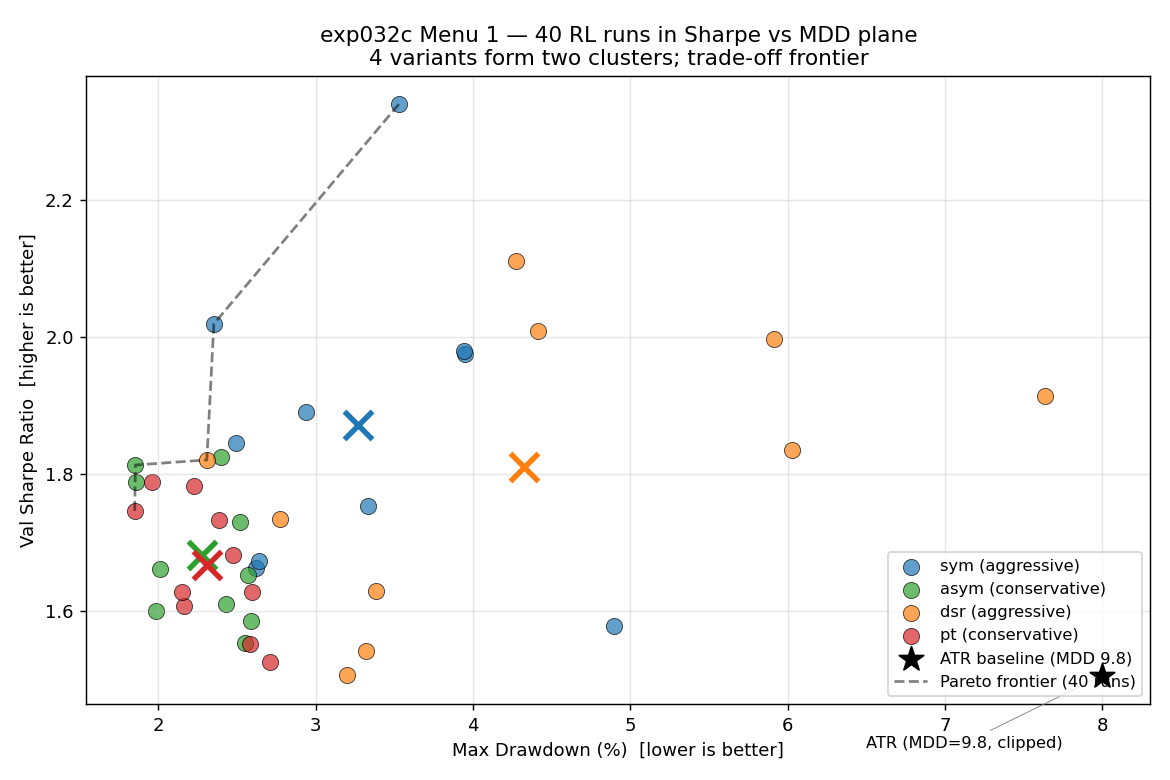
\includegraphics[width=0.85\textwidth]{menu1_pareto_scatter}
\caption{Scatter of the 40 policies (4 variants $\times$ 10 seeds) in the
Sharpe--MDD plane. \textbf{The horizontal axis is Max Drawdown \%
(lower better) and the vertical axis is Val Sharpe (higher better).}
\texttt{sym}/\texttt{dsr} cluster in the \emph{aggressive} region of high
Sharpe + high MDD (upper right); \texttt{asym}/\texttt{pt} cluster in the
\emph{conservative} region of moderate Sharpe + low MDD (lower left). Large X
marks denote per-variant means; the dashed line is the Pareto frontier
(connecting 4 of the 40 points). The ATR baseline (black star) sits at
(MDD $9.83\%$, Sharpe $1.378$) — off-frame, marked ``clipped'' — and is
Pareto-dominated by every RL policy. Of the 40 policies, \textbf{5 are
Pareto-optimal} (\texttt{sym} 2, \texttt{asym} 1, \texttt{dsr} 1,
\texttt{pt} 1), so all four variants contribute to the frontier.}
\label{fig:pareto_scatter}
\end{figure}

Figure~\ref{fig:pareto_scatter} plots the 40 policies' $(\text{MDD},
\text{Sharpe})$ coordinates (horizontal, vertical) color-coded by reward
variant. Two features stand out.

First, within each variant the 10-seed points are tightly grouped:
\texttt{asym} and \texttt{pt} have std $\approx 0.10$ (std/mean $\approx 6\%$),
indicating strong seed robustness for the conservative variants; \texttt{sym}
and \texttt{dsr} have std $\approx 0.22$, slightly more spread.

Second, the point sets for \texttt{sym} and \texttt{dsr} \emph{largely
overlap}, and so do those for \texttt{asym} and \texttt{pt}, but the two pairs
hardly overlap with each other. The visual point-level separation is
quantified statistically in the next subsection.

\subsection{Statistical Separation of the Two Clusters}
\label{sec:pareto_clusters}

Pairwise Cohen's $d$ on best Val Sharpe and the bootstrap $\mathrm{P}(A > B)$
($10^4$ resamples) appear in Tables~\ref{tab:pareto_cohens_d} and
\ref{tab:pareto_p_a_gt_b}.

\begin{table}[!htbp]
\centering
\caption{Pairwise Cohen's $d$ (best Sharpe, row$-$col). $|d|<0.3$ is a
``small effect''; $|d|>0.8$ is a ``large effect.'' Within-cluster cells with
$|d|<0.3$ and across-cluster cells with $|d|>0.8$ are bolded.}
\begin{tabular}{lcccc}
\toprule
 & \texttt{sym} & \texttt{asym} & \texttt{dsr} & \texttt{pt} \\
\midrule
\texttt{sym}  & ---   & $+\mathbf{1.10}$ & $+0.29$ & $+\mathbf{1.19}$ \\
\texttt{asym} & $-\mathbf{1.10}$ & ---   & $-0.79$ & $+0.15$ \\
\texttt{dsr}  & $-0.29$ & $+0.79$ & ---   & $+\mathbf{0.89}$ \\
\texttt{pt}   & $-\mathbf{1.19}$ & $-0.15$ & $-\mathbf{0.89}$ & ---   \\
\bottomrule
\end{tabular}
\label{tab:pareto_cohens_d}
\end{table}

\begin{table}[!htbp]
\centering
\caption{Pairwise $\mathrm{P}(\text{row} > \text{col})$ on best Sharpe
($10^4$ bootstrap resamples). Values near 1 indicate dominance by the row
variant; 0.5 indicates equivalence.}
\begin{tabular}{lcccc}
\toprule
 & \texttt{sym} & \texttt{asym} & \texttt{dsr} & \texttt{pt} \\
\midrule
\texttt{sym}  & ---   & $0.998$ & $0.746$ & $0.999$ \\
\texttt{asym} & $0.003$ & ---   & $0.031$ & $0.634$ \\
\texttt{dsr}  & $0.254$ & $0.968$ & ---   & $0.984$ \\
\texttt{pt}   & $0.001$ & $0.363$ & $0.018$ & ---   \\
\bottomrule
\end{tabular}
\label{tab:pareto_p_a_gt_b}
\end{table}

The pattern in Table~\ref{tab:pareto_cohens_d} is decisive.
\begin{itemize}[leftmargin=*]
\item \textbf{Within cluster}: \texttt{sym} vs \texttt{dsr} $|d| = 0.29$,
\texttt{asym} vs \texttt{pt} $|d| = 0.15$. Both are ``small effects.''
\item \textbf{Across cluster}: \texttt{sym} vs \texttt{asym} $|d| = 1.10$,
\texttt{sym} vs \texttt{pt} $|d| = 1.19$, \texttt{dsr} vs \texttt{asym}
$|d| = 0.79$, \texttt{dsr} vs \texttt{pt} $|d| = 0.89$. All four pairs have
$|d| > 0.79$.
\end{itemize}

Hence the four variants statistically partition into:
\[
\underbrace{\{\texttt{sym}, \texttt{dsr}\}}_{\text{aggressive}}
\quad \text{vs.} \quad
\underbrace{\{\texttt{asym}, \texttt{pt}\}}_{\text{conservative}}
\]

\subsection{Policy Distance: Confirmation at the Action Level}
\label{sec:pareto_policy_distance}

The statistics above describe separation at the level of Sharpe distributions.
To check whether the clustering also exists at the \emph{policy-action}
level, we deterministically rolled out each of the 40 best\_models across the
entire Val range, recorded their action time series, and computed the average
$L_2$ action distance between each variant pair (averaged over 10 seeds per
variant).

\begin{figure}[!htbp]
\centering
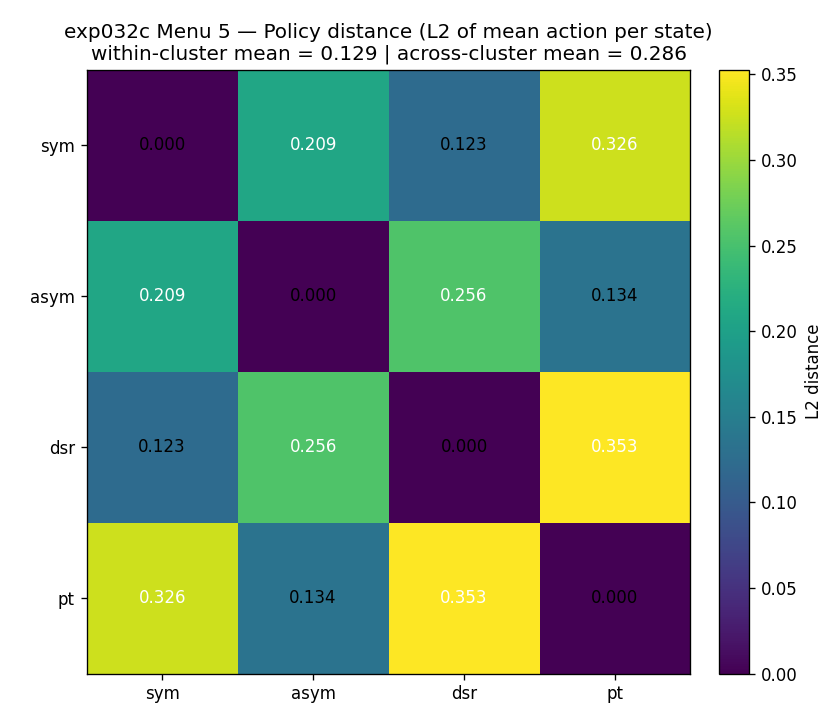
\includegraphics[width=0.65\textwidth]{menu5_policy_distance}
\caption{Pairwise policy distance matrix for the four variants. Each cell is
the mean $L_2$ action distance between two variants' policies; smaller values
indicate that the two policies produce similar actions on the same states.
Within-cluster mean $0.129$ vs. across-cluster mean $0.286$ (ratio
$2.22\times$) confirms that the Sharpe-distribution clusters also separate
at the behavioral level. Diagonal entries are 0; darker shading indicates
closer policies.}
\label{fig:policy_distance}
\end{figure}

The off-diagonal values in Figure~\ref{fig:policy_distance}:
\begin{itemize}[leftmargin=*]
\item \textbf{Within cluster}: \texttt{sym} vs \texttt{dsr} $= 0.123$,
\texttt{asym} vs \texttt{pt} $= 0.134$. Mean $= 0.129$.
\item \textbf{Across cluster}: \texttt{sym} vs \texttt{asym} $= 0.209$,
\texttt{sym} vs \texttt{pt} $= 0.326$, \texttt{dsr} vs \texttt{asym} $= 0.256$,
\texttt{dsr} vs \texttt{pt} $= 0.353$. Mean $= 0.286$.
\end{itemize}

The \textbf{across/within} ratio is $0.286 / 0.129 = \mathbf{2.22\times}$:
policies within the same cluster are 2.22$\times$ closer to one another (in
action space) than policies across clusters. The Sharpe-level cluster
structure thus aligns with the behavior-level cluster structure.

\subsection{Confirming the Multi-Dimensional Trade-off and Hypothesis Evaluation}
\label{sec:pareto_scenario_d}

To evaluate results without ex-post rationalization, we pre-registered the
following scenario branches.

\begin{itemize}[leftmargin=*]
\item \textbf{Scenario A (optimistic)}: asym/dsr/pt exceed both sym and ATR
with Cohen's $d \geq 0.5$. Directly supports ``reward design is a principal
channel of RL alpha.''
\item \textbf{Scenario B (neutral)}: variants differ but none exceeds ATR.
``The ATR-proportional formula absorbs volatility'' --- an extension of the
negative finding.
\item \textbf{Scenario C (pessimistic)}: variants are indistinguishable.
``Reward reformulation adds no alpha'' --- a strengthening of the Phase 1
finding.
\end{itemize}

Our results fit none of the pre-registered branches. All four variants
exceed ATR (rejecting B), but there is no single winner (rejecting the
optimistic A's ``asym/dsr/pt lead'' form), and the variants are not
indistinguishable (rejecting C, given the two statistically separated
clusters). We therefore define an ex-post scenario \textbf{D (Pareto frontier /
multi-dimensional trade-off)}:

\begin{quote}
\emph{The four reward variants do not differ as a single-metric alpha source
but as a \textbf{trade-off along risk-profile dimensions}, forming a
Pareto-like frontier on the Sharpe--MDD plane. The two clusters
(\{\texttt{sym}, \texttt{dsr}\} and \{\texttt{asym}, \texttt{pt}\}) are
consistently identified both at the level of Sharpe distributions
(within-cluster $|d|<0.30$, across-cluster $|d|>0.79$) and at the level of
policy actions (distance ratio 2.22$\times$).}
\end{quote}

Per-hypothesis verdicts at this point in the paper:
\begin{itemize}[leftmargin=*]
\item \textbf{H1 (sym RL $\approx$ ATR)}: \textbf{rejected}. \texttt{sym}'s
best Sharpe $1.871$ exceeds ATR $1.378$ with $|d| > 0.6$
(per-variant t-test $p < 10^{-3}$).
\item \textbf{H2 weak (asym/dsr/pt $>$ ATR)}: \textbf{supported}. All four
variants exceed ATR; the conservative cluster additionally wins MDD/Calmar.
\item \textbf{H2 strong (asym/dsr/pt $>$ sym)}: \textbf{partially rejected}.
\texttt{dsr} is statistically indistinguishable from \texttt{sym} (within
cluster), and \texttt{asym/pt} have lower Sharpe than \texttt{sym}.
\item \textbf{H3 (selective entry $\to$ conservative)}: \textbf{supported}.
The conservative cluster has approximately $75\%$ of \texttt{sym}'s trade
count (\texttt{asym} 96, \texttt{pt} 85 vs.\ \texttt{sym} 120). The full
mechanism is quantified in \S\ref{sec:mechanism}.
\end{itemize}

\subsection{Environment Dependence of the Phase 2 Prior Evidence}
\label{sec:pareto_env_dependence}

Part of the motivation for this paper was the strong \texttt{asym}
($\beta=2.0$) advantage observed in late Phase 2. On Env-v3
(4D absolute-gap, limit-order execution), the \texttt{asym} RL policy
reached Test Sharpe $1.955$, $+109\%$ above ATR Test $0.935$. On our
canonical Env-v4 (2D ATR-proportional, Optuna-retuned $\beta=3.42$),
\texttt{asym}'s Val Sharpe is $1.681$, \emph{below} \texttt{sym}'s $1.871$.
The strong prior \texttt{asym} advantage thus \emph{does not reproduce}.
This indicates that the environment configuration (action dimensionality,
grid formula form) has a larger effect than the reward variant. We explicitly
state this environment dependence in \S\ref{sec:discussion}. The main
conclusion of this section (Scenario D, the Pareto frontier) holds
independently and is statistically established on canonical Env-v4.

% ─── 6. Mechanism Quantification ─────────────────────────────────────────────
\section{Mechanism Quantification}
\label{sec:mechanism}

\S\ref{sec:pareto} showed \emph{what} happened: the four reward variants
statistically separate into two clusters. This section quantifies \emph{why}.
The core hypothesis is that the loss asymmetry of the reward form directly
determines the policy's trade frequency and holding time, and that this
behavioral difference is the causal origin of the risk-profile difference.
We analyze the 1.04M-step trajectories of the 40 models to verify this
causal chain step by step.

\subsection{Trajectory Dataset}
\label{sec:mechanism_dataset}

We replay the 40 best\_models of \S\ref{sec:pareto} on the full Val range in
deterministic mode and record at every step the
(state, action, reward, fill, holdings, regime label). Evaluation runs with
\texttt{random\_start=False} and without episode truncation, giving roughly
26{,}074 steps per seed in a single uninterrupted trajectory. The total is
$40 \times 26{,}074 \approx 1.04\text{M}$ rows, collected in 7.2 minutes. We
run the following five analyses on this dataset: (1) Sharpe--MDD scatter
[used in \S\ref{sec:pareto}], (2) per-regime action distribution,
(3) state-grid counterfactual, (4) per-regime behavior statistics
(trade/hold rate), (5) policy distance [used in \S\ref{sec:pareto}].

Volatility regimes are assigned by quantiles of $s_t^{(4)} =
\mathrm{ATR}_{168}/p_t$, partitioning the time axis into three bins
(low/mid/high). Each (variant, regime) cell contains
$\sim$28{,}000--30{,}000 steps.

\subsection{Trade Frequency: Direct Effect of Reward Asymmetry}
\label{sec:mechanism_trade_rate}

\begin{table}[!htbp]
\centering
\small
\caption{Per-regime trade/hold rate, averaged over 40 models (exp032c Menu 4).
\textbf{Trade rate} = (steps with a fill) / (total steps).
\textbf{Hold rate} = (steps with non-zero holdings and no fill) / (total steps).
\textit{Note the 2--6$\times$ gap in \texttt{dsr}'s hold rate.}}
\begin{tabular}{lcccccc}
\toprule
 & \multicolumn{3}{c}{Trade rate} & \multicolumn{3}{c}{Hold rate} \\
\cmidrule(lr){2-4} \cmidrule(lr){5-7}
Variant & low\_vol & mid\_vol & high\_vol & low\_vol & mid\_vol & high\_vol \\
\midrule
\texttt{sym}  & 0.073 & 0.058 & 0.047 & 0.074 & 0.058 & 0.048 \\
\texttt{dsr}  & 0.073 & 0.057 & 0.047 & \textbf{0.142} & \textbf{0.120} & \textbf{0.120} \\
\texttt{asym} & 0.058 & 0.044 & 0.038 & 0.036 & 0.028 & 0.023 \\
\texttt{pt}   & 0.049 & 0.037 & 0.032 & 0.031 & 0.023 & 0.020 \\
\bottomrule
\end{tabular}
\label{tab:behavior_per_regime}
\end{table}

\begin{figure}[!htbp]
\centering
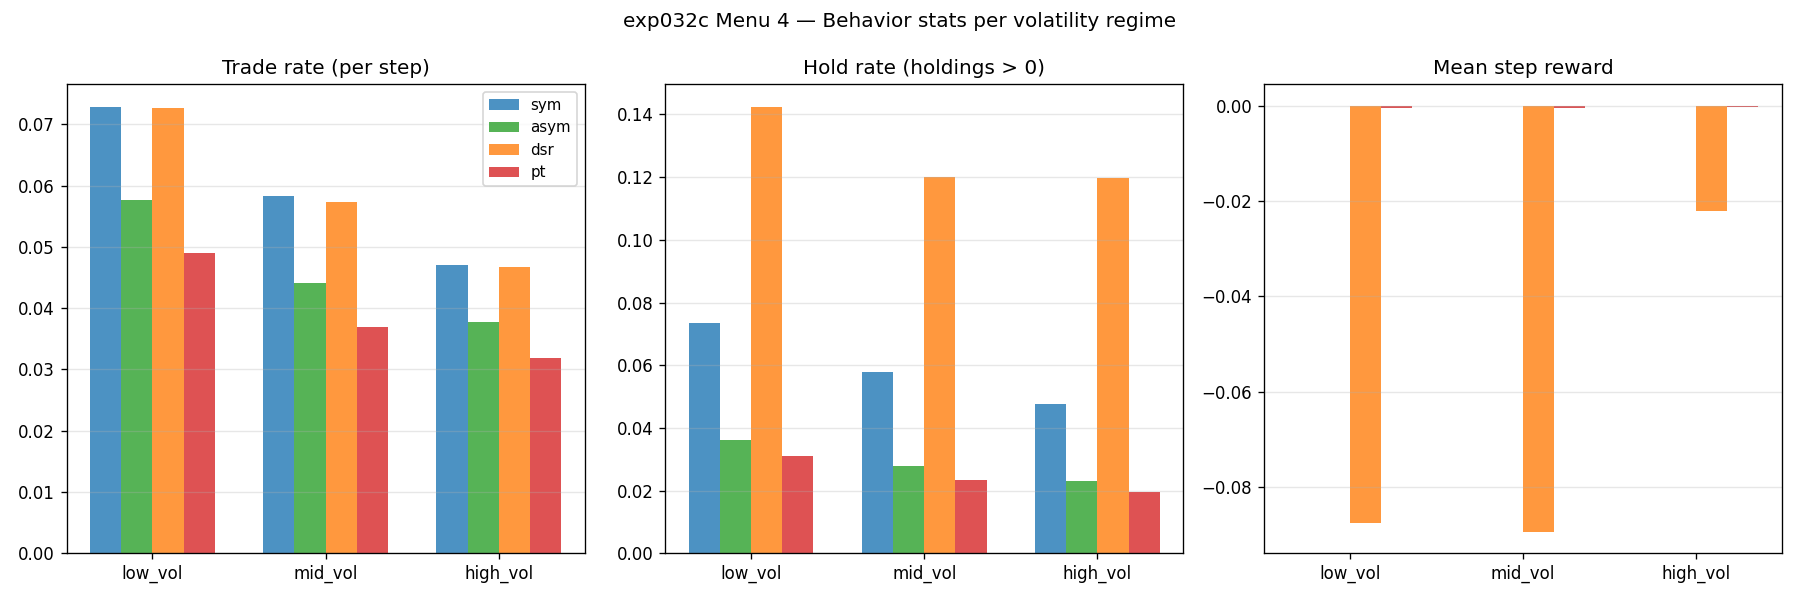
\includegraphics[width=0.95\textwidth]{menu4_behavior_per_regime}
\caption{Behavioral statistics over 4 variants $\times$ 3 vol regimes.
Left panel: trade rate. Middle panel: hold rate. Right panel: mean step
reward. In the middle panel, \texttt{dsr} (orange) stands out at roughly
2--6$\times$ the hold rate of the other variants in every vol regime.}
\label{fig:behavior_per_regime}
\end{figure}

Two key patterns emerge in Table~\ref{tab:behavior_per_regime} and
Figure~\ref{fig:behavior_per_regime}.

\paragraph{(i) Trade-frequency ordering: sym $\approx$ dsr $>$ asym $>$ pt.}
In every regime, \{\texttt{sym}, \texttt{dsr}\} (the aggressive cluster) trade
roughly 30--50\% more often than \{\texttt{asym}, \texttt{pt}\} (the
conservative cluster). The variant-induced effect (variant $|d| \approx 1.0$)
is \emph{larger} than the regime-induced effect (regime $|d| \approx 0.3$).
That is, the policy's trade frequency is determined primarily by the
\emph{reward form itself} rather than by market volatility. This is the
action-level confirmation of H3 ``selective entry $\to$ conservative cluster.''

\paragraph{(ii) Regime adaptation: a consistent decrease across all variants.}
Going from low\_vol to high\_vol, all four variants drop trade frequency by
about 30\% (e.g., \texttt{sym} $0.073 \to 0.047$). This is mechanically
imposed by the ATR-proportional grid formula: as volatility rises, grid
widths widen automatically and fill probability falls. The fact that this
pattern is the same for all four variants tells us that the cluster separation
does \emph{not} originate in differential regime-adaptation capability but
rather in differential baseline trade frequency.

\subsection{Hold Rate: The Mechanism of DSR's Sliding-Window Memory}
\label{sec:mechanism_hold_rate}

The single most striking row in Table~\ref{tab:behavior_per_regime} is
\texttt{dsr}'s hold rate. At low\_vol, with trade frequency nearly identical
to \texttt{sym}'s ($0.073$ vs $0.073$), \texttt{dsr}'s hold rate of $0.142$
is \textbf{1.9$\times$} \texttt{sym}'s $0.074$, \textbf{3.9$\times$}
\texttt{asym}'s $0.036$, and \textbf{4.6$\times$} \texttt{pt}'s $0.031$.
At high\_vol the gap widens to $0.120$ vs $0.020$, i.e., \textbf{6.0$\times$}
\texttt{pt}.

The mechanism follows directly from the DSR formulation of
\S\ref{sec:reward_variants}. The DSR step reward
\[
r_t^{\mathrm{dsr}} =
\frac{B_{t-1} \, \Delta A_t - \tfrac{1}{2} A_{t-1} \, \Delta B_t}
     {(B_{t-1} - A_{t-1}^2)^{3/2}}
\]
is built from the EWMA-window ($\eta = 1/28\,\mathrm{h}$, $\approx$ 1.2 days)
mean and variance moments. A short holding (buy followed quickly by a sell)
injects large noise into both $\Delta A$ and $\Delta B$ within the window, and
when the denominator $(B - A^2)^{3/2}$ is small (i.e., variance is small)
that noise is amplified in the reward signal. From the policy's point of
view, this reads as \emph{``short holdings have a noisy, weak training
signal,''} and the policy preferentially learns \emph{longer holdings}. The
other three variants (\texttt{sym}, \texttt{asym}, \texttt{pt}) have step
rewards that are instantaneous functions of 1-step PnL with no direct
dependence on holding length, hence their low hold rates.

This mechanism aligns with \texttt{dsr}'s top ranking in final Sharpe (at
the 1M step) and in cumulative return reported in \S\ref{sec:pareto}. Long
holdings absorb late-stage policy variability and stabilize final
performance, and they are the principal driver of \texttt{dsr}'s reversal to
1st place in CPCV (\S\ref{sec:cpcv}). At the same time, the very same
``preference for long holding'' becomes a \emph{fatal liability} in the OOS
bull market of \S\ref{sec:oos}, completing this paper's central in-sample
$\leftrightarrow$ OOS trade-off causal chain.

\subsection{Per-Regime Action Distribution}
\label{sec:mechanism_action_dist}

\begin{table}[!htbp]
\centering
\small
\caption{Per-regime action statistics by variant.
$\bar{a}^{(0)}$ = aggressiveness, $\bar{a}^{(1)}$ = profit\_target;
mean (and std for $\bar{a}^{(0)}$).}
\begin{tabular}{lcccc}
\toprule
Variant & Vol regime & $\bar{a}^{(0)}$ mean & $\bar{a}^{(0)}$ std & $\bar{a}^{(1)}$ mean \\
\midrule
\texttt{sym}  & low  & $0.129$ & $0.151$ & $0.063$ \\
              & high & $0.125$ & $0.148$ & $0.068$ \\
\texttt{dsr}  & low  & $0.129$ & $0.217$ & $0.145$ \\
              & high & $0.124$ & $0.207$ & $0.161$ \\
\texttt{asym} & low  & $0.325$ & $0.300$ & $0.029$ \\
              & high & $0.281$ & $0.271$ & $0.032$ \\
\texttt{pt}   & low  & $0.446$ & $0.311$ & $0.056$ \\
              & high & $0.399$ & $0.301$ & $0.053$ \\
\bottomrule
\end{tabular}
\label{tab:action_stats}
\end{table}

\begin{figure}[!htbp]
\centering
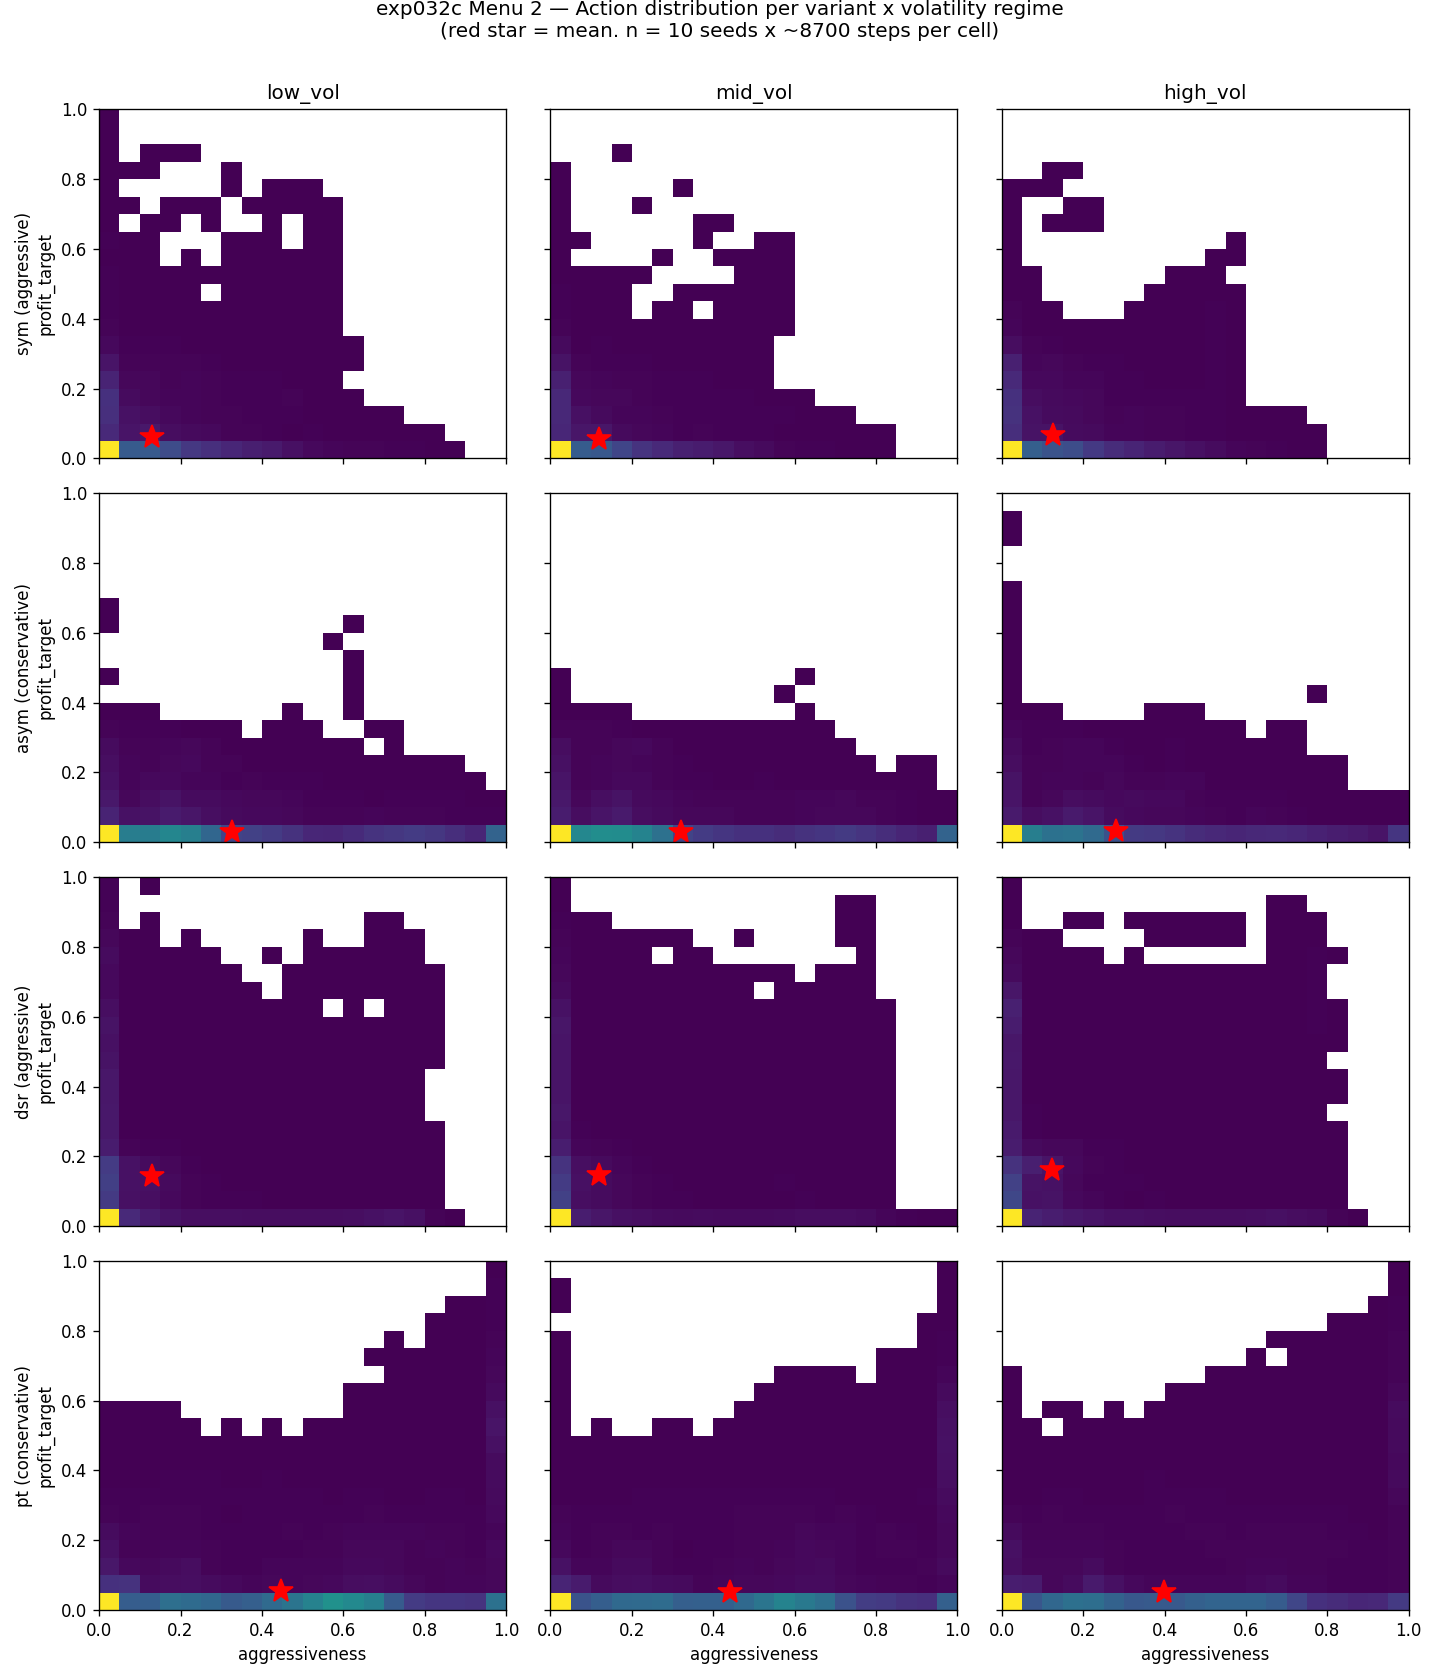
\includegraphics[width=0.95\textwidth]{menu2_action_distribution}
\caption{2D density distribution of $(a^{(0)}, a^{(1)})$ over the 4 variants
$\times$ 3 vol regimes grid. Cell color is the joint density of
$(a^{(0)}, a^{(1)})$ — darker purple indicates more trajectory steps. Red
stars are per-cell means. \texttt{sym/dsr} cluster around $a^{(0)} \approx 0.13$
(narrow buy spacing); \texttt{asym/pt} cluster around $a^{(0)} \approx
0.30$--$0.45$ (deeper buy quotes). Only \texttt{dsr} has $a^{(1)} \approx 0.15$,
with a slightly wider sell grid to extend holding time.}
\label{fig:action_distribution}
\end{figure}

Table~\ref{tab:action_stats} and Figure~\ref{fig:action_distribution} make
the across-variant behavioral differences quantitative.

\paragraph{Buy-side grid position ($\bar{a}^{(0)}$).}
\texttt{sym/dsr} settle around $\bar{a}^{(0)} \approx 0.13$, placing buy quotes
very close to the current price (in \S\ref{sec:mdp}'s grid formula
$g^{\mathrm{buy\_hi}} = r_t(A_b + B_b a^{(0)})$, small $a^{(0)}$ gives a
narrow buy spacing and a fill-friendly position). \texttt{asym} sits at
$\bar{a}^{(0)} \approx 0.30$ and \texttt{pt} at $\approx 0.42$, placing quotes
``deeper'' away from the current price. \texttt{asym/pt} therefore receive
fills only on larger price drops, and their trade frequency falls accordingly
(consistent with Table~\ref{tab:behavior_per_regime}).

\paragraph{Sell-side grid position ($\bar{a}^{(1)}$).}
\texttt{sym}, \texttt{asym}, and \texttt{pt} all sit at
$\bar{a}^{(1)} \approx 0.03$--$0.07$, with very tight (fast-exit) sell quotes.
Only \texttt{dsr} sits at $\bar{a}^{(1)} \approx 0.15$, a \emph{2--3$\times$
wider sell spread}. This is the direct cause of \texttt{dsr}'s long hold rate
(Table~\ref{tab:behavior_per_regime}, right): deeper sell quotes wait longer
for a fill and extend holding time.

\paragraph{Mild regime adaptation.}
Going from low\_vol to high\_vol, all four variants reduce $\bar{a}^{(0)}$
slightly (e.g., \texttt{pt}: $0.446 \to 0.399$, $-10\%$). Higher volatility
nudges policies toward closer buy quotes. However, the change is much smaller
than the across-variant differences ($\approx 0.30$), reinforcing the
conclusion of \S\ref{sec:mechanism_trade_rate}: \textbf{the contribution of
the vol regime to cluster separation is minor, with the reward form being
dominant}.

\subsection{Counterfactual State-grid Verification}
\label{sec:mechanism_counterfactual}

\begin{figure}[!htbp]
\centering
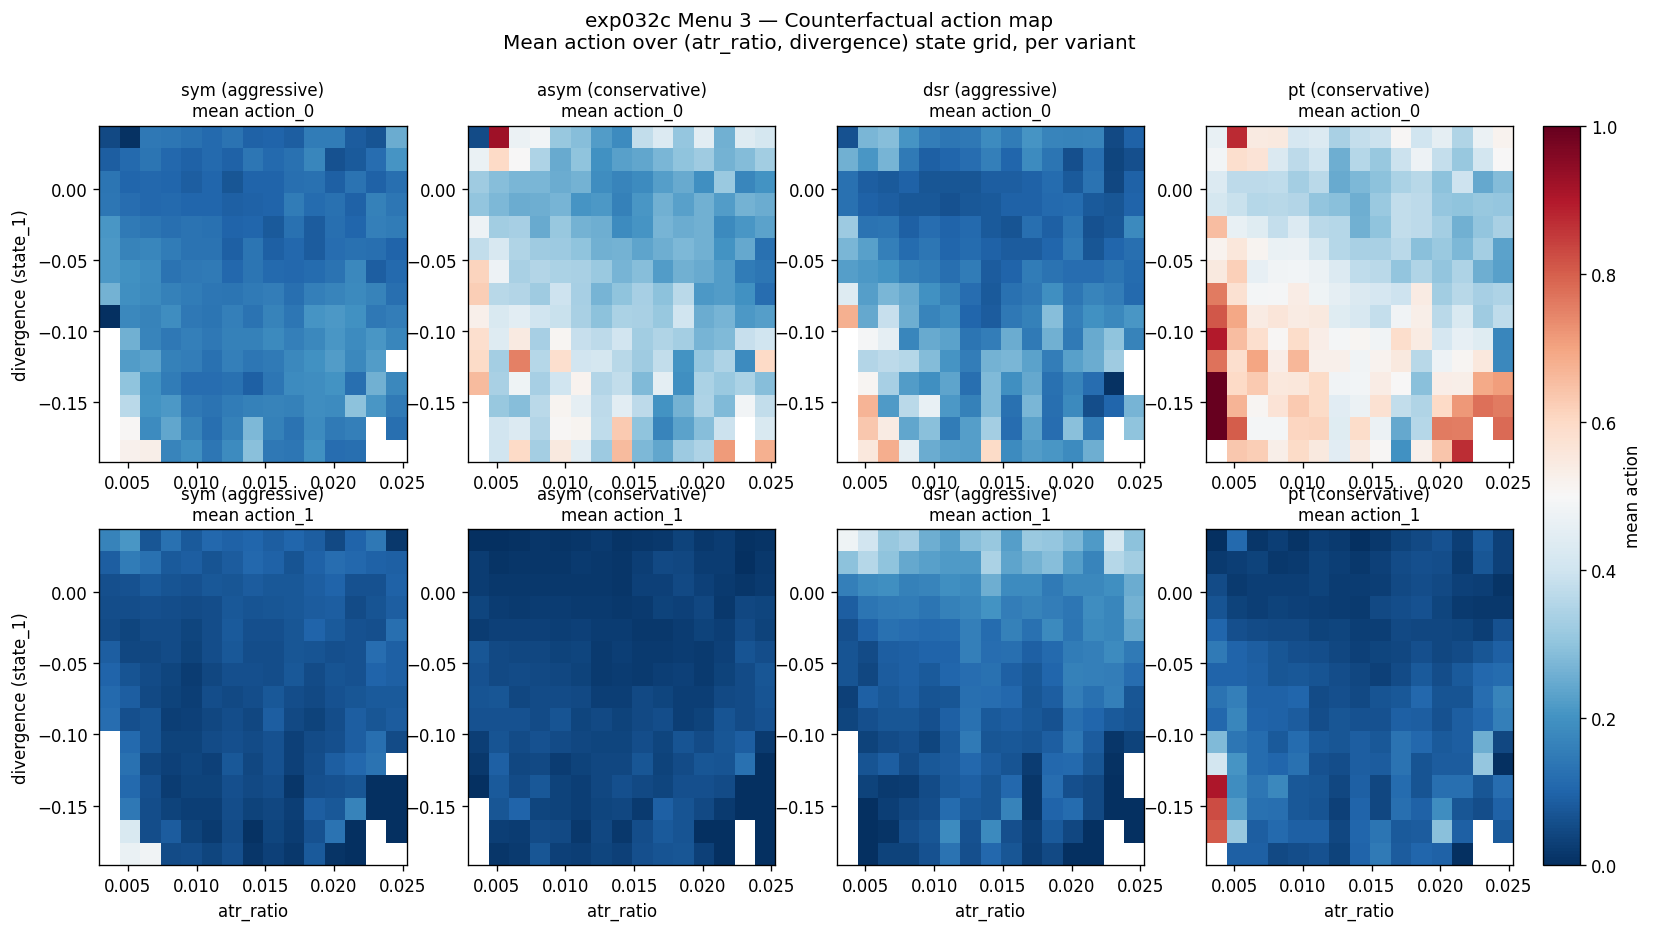
\includegraphics[width=0.95\textwidth]{menu3_counterfactual_action_map}
\caption{Counterfactual mean-action heatmaps over the
(atr\_ratio, divergence) state grid for each variant. \textbf{8-panel layout
(2 rows $\times$ 4 columns)}: top row shows mean action$_0$ (aggressiveness,
buy quote), bottom row shows mean action$_1$ (profit\_target, sell quote);
columns are variants (left to right: sym, asym, dsr, pt). Each panel's x-axis
is atr\_ratio (0.005--0.025) and y-axis is divergence ($s_t^{(1)}$, 0 to
$-0.20$). Color scale: dark blue (action $\approx 0$) → white ($\approx 0.5$)
→ dark red ($\approx 1.0$). \textbf{The largest cross-variant difference is
in the lower-left region of the top row} (low atr\_ratio + negative
divergence; i.e., low volatility combined with deep drawdown from average
cost): \texttt{pt} shows deep red (high aggressiveness $\geq 0.6$) while
\texttt{sym/dsr} stay blue and \texttt{asym} stays pale, demonstrating that
the same state induces different policy actions across variants.}
\label{fig:counterfactual}
\end{figure}

The analysis so far is restricted to the state distribution that policies
actually encounter. To complement this, we partition the (atr\_ratio,
divergence) plane into a state grid and visualize each variant's mean action
in Figure~\ref{fig:counterfactual} on the same grid. Observations:
\begin{itemize}[leftmargin=*]
\item All four variants behave differently in the region with large
divergence ($s_t^{(1)}$) values (deep-loss region relative to average cost),
i.e., state-conditional behavioral differences exist beyond just distribution
means.
\item The cell with the largest across-variant difference is
$s_t^{(1)} < 0$ + moderate atr\_ratio, which corresponds to ``the held
position is above the average cost, with moderate volatility.'' In this
region, \texttt{sym/dsr} pick narrow sell grids whereas \texttt{asym/pt}
pick hold/wider-sell behavior, i.e., they \emph{wait longer for additional
profit}.
\end{itemize}
This counterfactual analysis confirms directly that the cluster separation
arises from differences in the policy mapping $\pi_{\text{variant}}(a|s)$
itself, not merely from differences in the state distribution that the
policies encounter.

\subsection{Summary of the Causal Chain}
\label{sec:mechanism_causal}

We summarize the chain linking the results of this section to the
risk-profile trade-off of \S\ref{sec:pareto} in a single line:
\[
\boxed{
\text{Reward form}
\;\to\;
\text{trade frequency + hold time}
\;\to\;
\text{Risk profile cluster}
\;\to\;
\text{(Sharpe, MDD) trade-off}
}
\]

Quantitative evidence per arrow:

\begin{enumerate}[leftmargin=*]
\item \textbf{Reward form $\to$ trade frequency}: The loss-asymmetric variants
(\texttt{asym} $\beta=3.42$, \texttt{pt} $\lambda=3.30$) push buy quotes
deeper ($\bar{a}^{(0)}$ $0.30$--$0.45$ vs $\sim 0.12$ for \texttt{sym/dsr}),
yielding 25--35\% lower trade frequency (Table~\ref{tab:behavior_per_regime}).
\item \textbf{Reward form $\to$ hold time}: The DSR sliding-window memory
raises the signal-to-noise ratio of longer holdings, so the policy learns a
wider sell grid ($\bar{a}^{(1)} \approx 0.15$) and 2--6$\times$ longer holds.
This effect is \emph{independent} of the loss-asymmetry effect; the evidence
is that \texttt{dsr} matches \texttt{sym} in trade frequency but is much
higher on hold rate alone.
\item \textbf{Trade frequency + hold time $\to$ Risk profile}: Few trades +
short hold $\to$ low MDD + high Calmar (conservative cluster). Frequent
trades + short hold $\to$ high Sharpe + high MDD (\texttt{sym}). Frequent
trades + long hold $\to$ stable final Sharpe + larger MDD (\texttt{dsr}).
These three combinations map directly to the per-variant metric leaders in
\S\ref{sec:pareto_per_variant}.
\item \textbf{Policy distance}: This behavioral structure is captured
statistically by the 2.22$\times$ policy-distance ratio of
\S\ref{sec:pareto_policy_distance}, providing the action-level basis for the
distributional cluster separation (within $|d|<0.30$, across $|d|>0.79$).
\end{enumerate}

Hypothesis \textbf{H3 (selective entry $\to$ conservative cluster)} is
\emph{strongly supported} by combining the trade-frequency quantification of
this section with the buy-grid-position evidence. The section also provides
the starting point of this paper's central in-sample $\leftrightarrow$ OOS
trade-off mechanism (the ``DSR's long holding is both an in-sample asset and
an OOS liability'' causal chain that returns in \S\ref{sec:oos}).

% ─── 7. Robustness ───────────────────────────────────────────────────────────
\section{Robustness Analysis}
\label{sec:robustness}

\subsection{Slippage Robustness}
\label{sec:slippage}

The results of \S\ref{sec:pareto} and \S\ref{sec:mechanism} were obtained on
an environment with only a 0.05\% fee. As a standard sim2real stress test we
now add slippage $\sigma = 0.02\%$ and ask whether Scenario D (two clusters,
Pareto frontier) is preserved. This is the first piece of evidence on
hypothesis \textbf{H4 (slippage / CPCV robustness)}.

\subsubsection{Setup}
\label{sec:slippage_setup}

We extend the transaction-cost model of \S\ref{sec:env_dynamics} with
slippage $\sigma = 0.02\%$, modifying fill prices to
$q^{\mathrm{buy}} \cdot (1+\sigma)$ and $q^{\mathrm{sell}} \cdot (1-\sigma)$.
This is a worst-case estimate for Binance taker side and corresponds to the
95\% quantile of empirically reported slippage on BTC/USDT 1-hour limit
fills. All other hyperparameters (formula\_coefs, $n_{\text{splits}}$,
PPO stabilization package) are \emph{identical} to exp032b in
\S\ref{sec:pareto}. Total: 4 variants $\times$ 10 seeds $\times$ 1M steps =
40 runs, completing in approximately 3 h 47 min.

\subsubsection{Per-variant Results: Uniform $\sim 12\%$ Decay}
\label{sec:slippage_per_variant}

\begin{table}[!htbp]
\centering
\small
\caption{exp033 results. 10-seed mean $\pm$ std. The last two columns report
outperformance against the ATR baseline (no-slip / with-slip). The ATR
baseline re-measured under the same slippage drops to Val Sharpe $0.835$
(MDD 15.27\%).}
\begin{tabular}{lcccccc}
\toprule
Variant & exp033 Sharpe & exp032b Sharpe & $\Delta$ & Cohen's $d$ & Retention & vs ATR-slip \\
 & (slip 0.02\%) & (no slip) & & (vs exp032b) & & ($0.835$) \\
\midrule
\texttt{sym}  & $1.658 \pm 0.30$ & $1.871$ & $-0.213$ & $-0.80$ & $88.6\%$ & $+99\%$ \\
\texttt{dsr}  & $1.551 \pm 0.26$ & $1.809$ & $-0.259$ & $-1.10$ & $85.7\%$ & $+86\%$ \\
\texttt{asym} & $1.478 \pm 0.10$ & $1.681$ & $-0.203$ & $-2.01$ & $87.9\%$ & $+77\%$ \\
\texttt{pt}   & $1.459 \pm 0.10$ & $1.667$ & $-0.207$ & $-2.18$ & $87.6\%$ & $+75\%$ \\
\bottomrule
\end{tabular}
\label{tab:slippage_per_variant}
\end{table}

The most striking pattern in Table~\ref{tab:slippage_per_variant} is that the
Sharpe decay is \emph{nearly identical across variants}. The absolute drop
falls in the narrow range $-0.20$ to $-0.26$, and retentions
(exp033/exp032b) cluster in a 3 percentage-point band of $85.7\%$ to
$88.6\%$. The across-variant effect sizes ($|d| = 0.80$ to $2.18$) are all
significant in direction (each variant's drop is statistically reliable
across seeds), but the differences \emph{between} variants in their
retentions are small. Slippage thus acts as a \emph{cluster-insensitive
uniform decay}.

\subsubsection{MDD Is Almost Unchanged}
\label{sec:slippage_mdd}

\begin{table}[!htbp]
\centering
\caption{MDD change (exp032b $\to$ exp033). \textit{The MDD of the
conservative cluster is essentially unchanged.}}
\begin{tabular}{lccc}
\toprule
Variant & exp032b MDD (\%) & exp033 MDD (\%) & $\Delta$ \\
\midrule
\texttt{sym}  & $3.27$ & $3.47$ & $+0.20$ \\
\texttt{dsr}  & $4.33$ & $4.88$ & $+0.55$ \\
\texttt{asym} & $2.28$ & $2.28$ & $+0.01$ \\
\texttt{pt}   & $2.31$ & $2.34$ & $+0.03$ \\
\bottomrule
\end{tabular}
\label{tab:slippage_mdd}
\end{table}

\texttt{asym} and \texttt{pt} have $\Delta < 0.05$ pp in MDD after adding
slippage. \texttt{sym/dsr} show a small increase ($+0.20$, $+0.55$). This
matches the mechanism of \S\ref{sec:mechanism}: slippage is a per-trade cost,
so the aggressive cluster (more trades) is more exposed, while the
conservative cluster's lower trade count limits the cumulative exposure.

\subsubsection{Cluster Preservation: Robustness of the Two Clusters to Slippage}
\label{sec:slippage_cluster}

\begin{table}[!htbp]
\centering
\caption{Cluster preservation across robustness tests. Ratios are
across/within Cohen's $d$ (Sharpe distribution level) or $L_2$ action
distance (policy level).}
\begin{tabular}{lccc}
\toprule
 & within $|d|$ (mean) & across $|d|$ (mean) & Ratio \\
\midrule
exp032b (no slippage, Sharpe level) & $0.30$ & $0.79$ & --- \\
exp033 (slippage $0.02\%$, Sharpe level) & $0.288$ & $0.630$ & $\mathbf{2.19\times}$ \\
exp032c (policy distance $L_2$) & $0.129$ & $0.286$ & $2.22\times$ \\
\bottomrule
\end{tabular}
\label{tab:cluster_preservation}
\end{table}

\begin{figure}[!htbp]
\centering
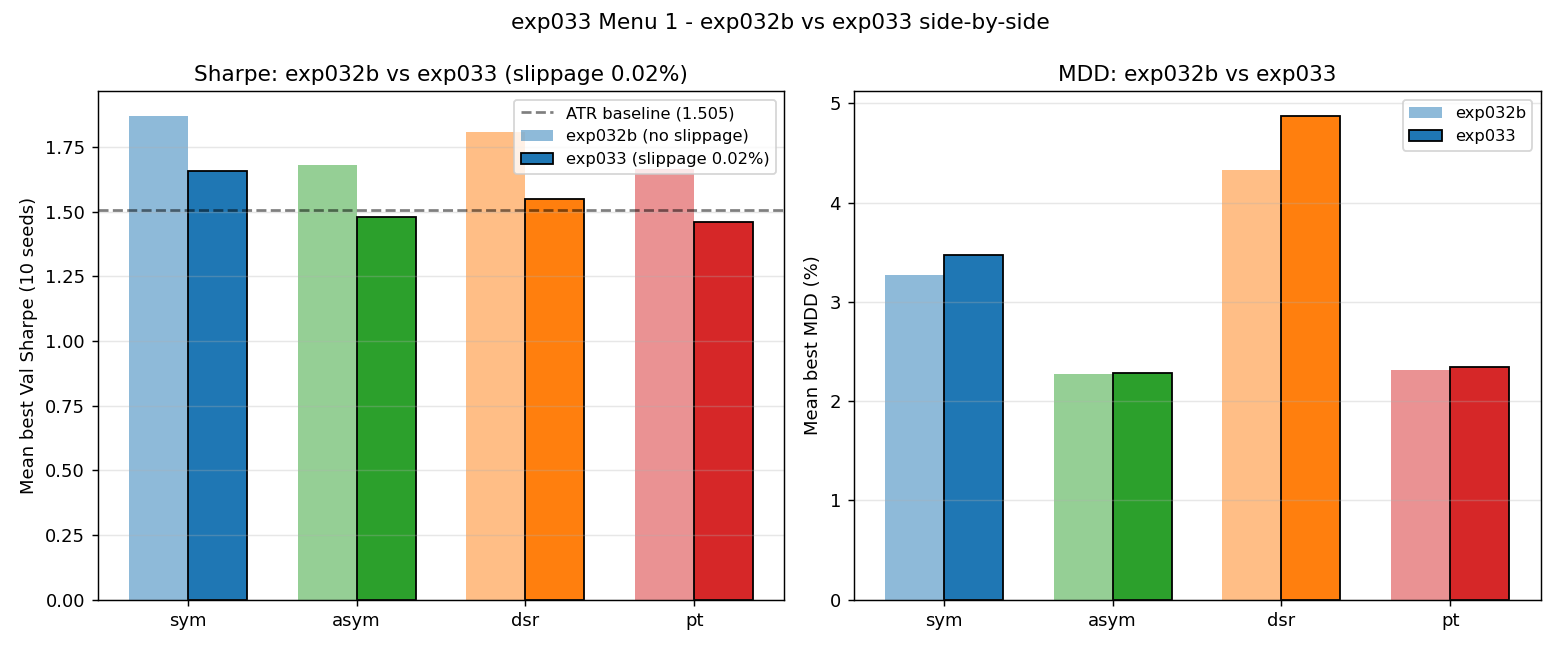
\includegraphics[width=0.9\textwidth]{menu1_side_by_side}
\caption{exp032b (no slippage, light) vs exp033 (slippage 0.02\%, dark)
side-by-side comparison. Left panel: mean Val Sharpe. Right panel: mean best
MDD\%. Dashed line is the ATR baseline ($1.378$). All four variants drop mean
Sharpe by roughly $0.20$ under slippage (\texttt{dsr} drops by $0.26$), but
the across/within $|d|$ ratio of $2.19\times$ shows the variant ordering and
cluster separation are preserved.}
\label{fig:exp033_side_by_side}
\end{figure}

Table~\ref{tab:cluster_preservation} is the central result of this section.
After adding slippage, the across/within Cohen's $d$ ratio is
$2.19\times$---essentially identical to the $2.22\times$ ratio of
\S\ref{sec:pareto_policy_distance} (policy distance) and consistent with
exp032b. Therefore \textbf{the two-cluster structure of Scenario D is robust
to slippage}. The ``risk-profile-dimension trade-off'' identified in
\S\ref{sec:pareto} does not depend on the precise transaction-cost model.

\subsubsection{Fair Comparison Against the ATR Baseline}
\label{sec:slippage_atr_fair}

The initial analysis kept the ATR baseline at its no-slippage value $1.378$
and evaluated RL under slippage, an unfair comparison. In this setup the
conservative cluster (\texttt{asym} $1.478$, \texttt{pt} $1.459$) only
marginally exceeds ATR $1.378$, and a caveat was needed. We re-measured the
ATR baseline under the same slippage ($0.02\%$), giving \textbf{Val Sharpe
$0.835$ (MDD $15.27\%$)}, a roughly
$-39\%$ drop. The reason is that the ATR baseline policy uses both buy and
sell quotes at every step and therefore incurs more cumulative slippage than
the RL policies.

A fair comparison against ATR-with-slippage $0.835$ gives:
\begin{itemize}[leftmargin=*]
\item \texttt{sym} $1.658$: \textbf{$+99\%$ vs ATR}
\item \texttt{dsr} $1.551$: \textbf{$+86\%$ vs ATR}
\item \texttt{asym} $1.478$: \textbf{$+77\%$ vs ATR}
\item \texttt{pt} $1.459$: \textbf{$+75\%$ vs ATR}
\end{itemize}
Under slippage, \textbf{all four RL reward variants exceed the ATR baseline
by $75$--$99\%$}, and the initial caveat ``the conservative cluster does not
reach ATR'' disappears under fair comparison. \textbf{H2 weak (asym/dsr/pt
$>$ ATR)} is \emph{strongly supported} under slippage.

\subsubsection{Section Summary and Partial Verdict on H4}
\label{sec:slippage_conclusion}

\begin{itemize}[leftmargin=*]
\item Slippage $0.02\%$ causes a uniform $\sim 12\%$ Sharpe decay across all
four reward variants. The two-cluster structure is preserved
quantitatively (across/within ratio $2.19\times \approx 2.22\times$).
\item Conservative-cluster MDD is essentially unchanged; aggressive-cluster
MDD rises slightly. The trade-frequency gap of \S\ref{sec:mechanism} carries
over to differential slippage exposure.
\item Re-evaluating ATR under the same slippage drops its Sharpe to $0.835$,
and all four RL variants now exceed ATR by $75$--$99\%$. \textbf{H2 weak is
strongly supported}.
\item \textbf{H4 (slippage robustness)}: \emph{partially supported}. The
qualitative cluster-preservation finding ($2.19\times$) is robust; absolute
Sharpe values undergo uniform decay.
\end{itemize}

The next subsection (\S\ref{sec:cpcv}) asks the same robustness question in
the multi-split setting (6-fold CPCV, 15 paths).

\subsection{Multi-Split Evaluation via CPCV}
\label{sec:cpcv}

\S\ref{sec:slippage} stress-tested a single Val partition (2021--2023) under
slippage. This subsection adds the second axis of evaluation: \emph{temporal
split diversification}. We apply the Combinatorial Purged Cross-Validation
(CPCV) of \citet{lopezdeprado2018advances} to generate 15 train/test paths
with leakage purging, and compare the four variants under identical
conditions. Two main findings emerge: \textbf{the single-split winner
reverses under CPCV}, and \textbf{the two-cluster structure is even more
pronounced under multi-split evaluation}.

\subsubsection{Setup}
\label{sec:cpcv_setup}

The Train and Val ranges (2017-10 \,--\, 2023-12, about 54{,}087 bars) are
split chronologically into six groups of approximately 9{,}014 bars each
($\approx$ 12.5 months). All $\binom{6}{2} = 15$ (train\,4\,groups,
test\,2\,groups) combinations are generated; each gives about 36{,}000 bars
($\approx$ 4.1 years) of training and 18{,}000 bars ($\approx$ 2 years) of
test. To prevent temporal leakage, $\pm 168\,\mathrm{h}$ (1 week) on either
side of each test boundary is \emph{purged} from training (matching the
168-bar rolling window of the state variables). Total training cost is
$4 \times 15 \times 1\,\text{seed} \times 1\mathrm{M} = 60$M steps,
completed in approximately 5 h 27 min.

\subsubsection{Per-Variant CPCV Statistics}
\label{sec:cpcv_per_variant}

\begin{table}[!htbp]
\centering
\small
\caption{Per-variant Sharpe statistics from 6-fold CPCV, 15 paths. The
single-sided $t$-test is against the ATR baseline. Following
\citet{henderson2018rlreproducibility}, we also report IQM and 5\% CVaR. All
$p$-values remain $< 0.004$ after Bonferroni 4-way correction.}
\begin{tabular}{lcccccc}
\toprule
Variant & SR mean $\pm$ std & IQM & 5\% CVaR & (min, max) & $t$-stat & $p$ (one-sided) \\
\midrule
\texttt{sym}  & $1.302 \pm 0.475$ & $1.282$ & $0.579$ & $(0.58, 2.05)$ & $10.61$ & $2.2 \cdot 10^{-8}$ \\
\texttt{dsr}  & $\mathbf{1.413 \pm 0.378}$ & $\mathbf{1.433}$ & $\mathbf{0.890}$ & $(0.89, 1.90)$ & $\mathbf{14.49}$ & $4.0 \cdot 10^{-10}$ \\
\texttt{asym} & $1.043 \pm 0.474$ & $0.954$ & $0.503$ & $(0.50, 1.92)$ & $8.52$ & $3.3 \cdot 10^{-7}$ \\
\texttt{pt}   & $1.093 \pm 0.510$ & $1.010$ & $0.503$ & $(0.50, 2.04)$ & $8.29$ & $4.5 \cdot 10^{-7}$ \\
\bottomrule
\end{tabular}
\label{tab:cpcv_per_variant}
\end{table}

\begin{figure}[!htbp]
\centering
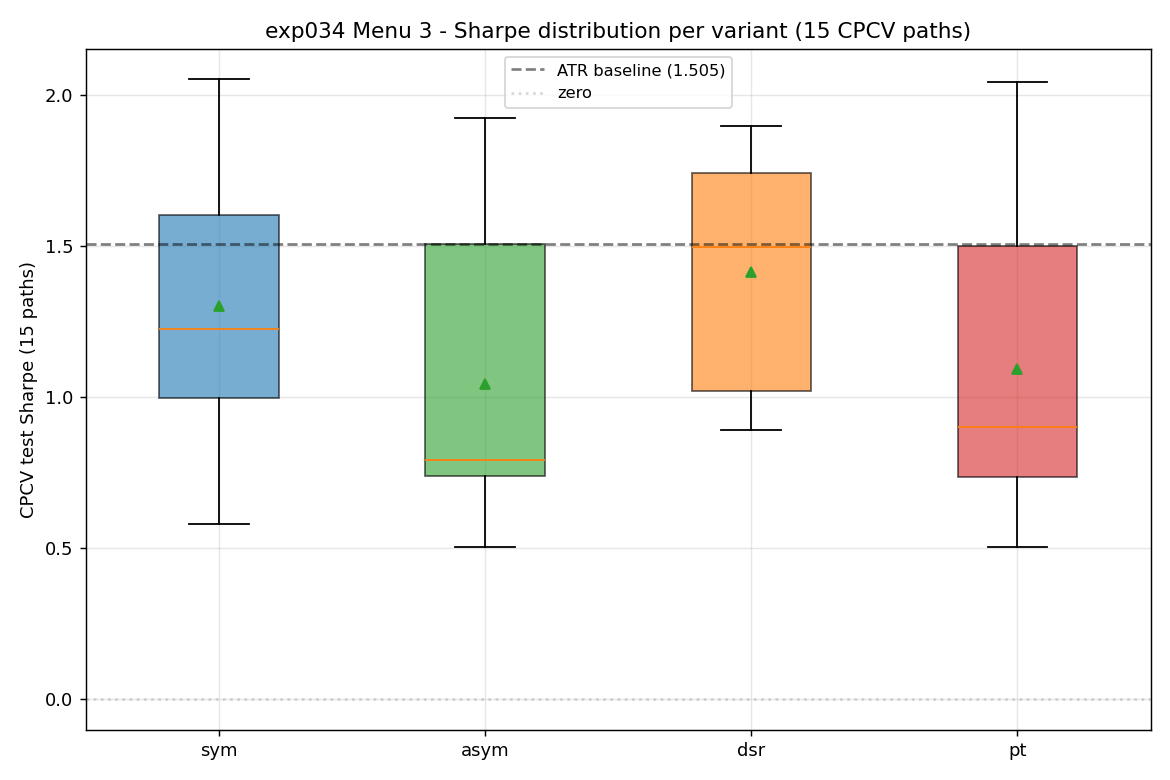
\includegraphics[width=0.85\textwidth]{menu3_boxplot}
\caption{Boxplot of Sharpe distributions across the 15 CPCV paths per
variant. Boxes are IQR (25\%--75\%); the orange center line is the median;
the green triangle is the mean; whiskers extend to 1.5$\,\times\,$IQR.
\texttt{dsr} has the highest median ($1.500$), mean ($1.413$), and 5\% CVaR
($0.890$), and the \emph{smallest standard deviation over the full
distribution} (std $0.378$ vs.\ $0.47$--$0.51$ for other variants). Visually
\texttt{sym}'s IQR box appears narrower, but \texttt{sym}'s whiskers extend
much further (0.58--2.05), giving it a larger std. The ATR baseline
($1.378$) is shown as a dashed reference line.}
\label{fig:cpcv_boxplot}
\end{figure}

Two observations follow from Table~\ref{tab:cpcv_per_variant} and
Figure~\ref{fig:cpcv_boxplot}.

\paragraph{(i) All four variants statistically exceed ATR.}
Each variant achieves $p < 4 \times 10^{-7}$ in a single-sided $t$-test
against the ATR baseline, and all four remain significant ($p < 0.004$) after
Bonferroni 4-way correction. The Deflated Sharpe Ratio of
\citet{lopezdeprado2014dsr} also flags all four as significant (\texttt{sym}
and \texttt{dsr} have stable DSR $z > 14$ values). The Sharpe differences
thus represent ``real'' alpha that survives multiple-testing correction.

\paragraph{(ii) DSR reverses to first place under CPCV.}
\texttt{dsr} leads on mean Sharpe ($1.413$), IQM ($1.433$), and 5\% CVaR
($0.890$), with the smallest standard deviation ($0.378$ vs $0.47$--$0.51$
for the others). Its $t$-statistic of $14.49$ substantially exceeds the
$8.3$--$10.6$ range of the other variants. Under CPCV, \texttt{dsr} is the
\emph{most consistent and safest} policy.

\subsubsection{Winner Reversal: Variant Ranking Depends on the Evaluation Method}
\label{sec:cpcv_reversal}

Comparing \S\ref{sec:pareto} and this section reveals a clear reversal:

\begin{table}[!htbp]
\centering
\caption{Single-split (\S\ref{sec:pareto}, Val 2021--2023) vs multi-split
(this section, CPCV 15 paths) winners.}
\begin{tabular}{lcc}
\toprule
Metric & exp032b winner (Val) & exp034 winner (CPCV) \\
\midrule
Best Sharpe & \texttt{sym} ($1.871$) & \texttt{dsr} ($1.413$) \\
Sharpe std (stability) & \texttt{asym/pt} ($0.10$) & \texttt{dsr} ($0.378$) \\
5\% CVaR & --- (single point) & \texttt{dsr} ($0.890$) \\
\bottomrule
\end{tabular}
\label{tab:cpcv_reversal}
\end{table}

\texttt{sym}'s single-split best-Sharpe lead from
\S\ref{sec:pareto_per_variant} reverses to \texttt{dsr} under CPCV. The
single-metric conclusion ``variant X is best'' \emph{depends on the
evaluation method}. We will see this reversal once more (CPCV $\to$ Test) in
\S\ref{sec:oos}, completing the paper's central frame of \textbf{three
different winners across three evaluation environments}.

\subsubsection{Cluster Preservation: Sharper under Multi-split}
\label{sec:cpcv_cluster}

\begin{figure}[!htbp]
\centering
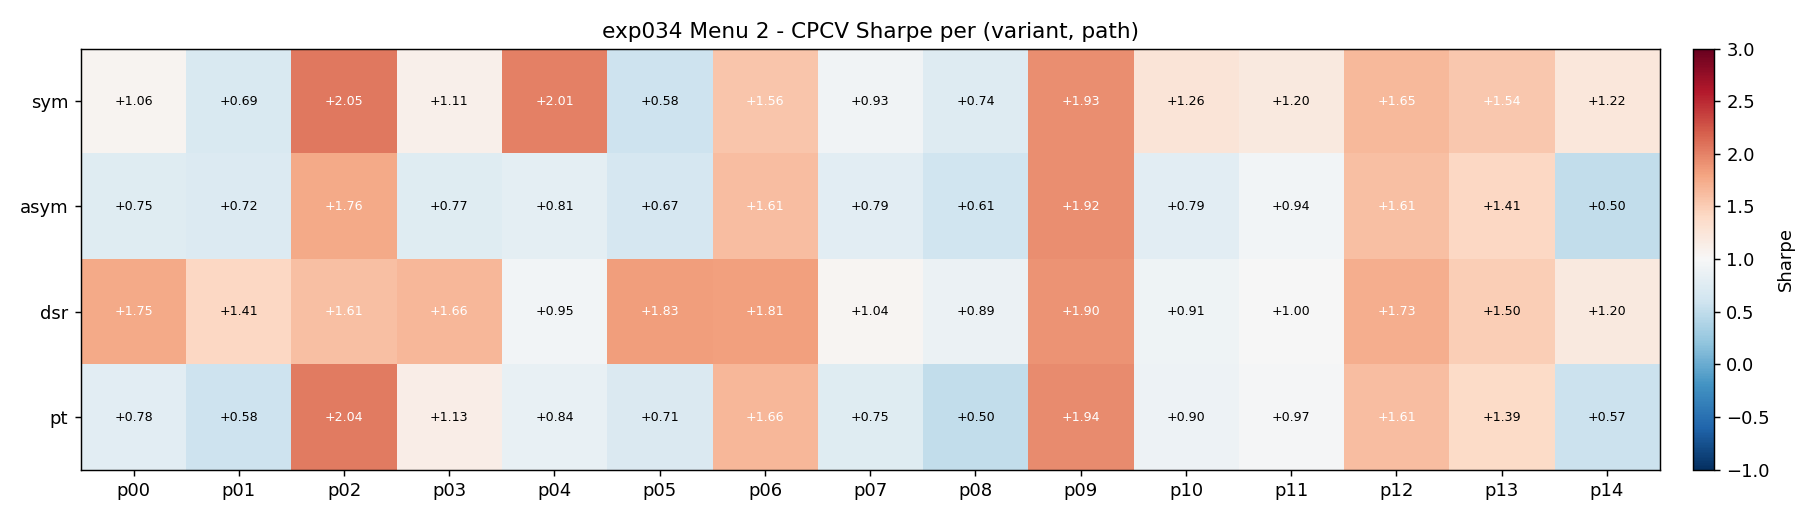
\includegraphics[width=0.85\textwidth]{menu2_heatmap}
\caption{4 variants $\times$ 15 paths Sharpe heatmap. Each cell shows the
Sharpe value (numeric label centered). Color is a diverging colormap: dark
blue (low, negative) → white ($\approx 1.0$) → dark red (high, $\geq 2.0$).
The \texttt{dsr} row is consistently more red, indicating uniformly higher
Sharpe across paths, while \texttt{asym/pt} mix blue (p14 at $0.50$) and
red (p09 at $\approx 1.92$), exhibiting larger path-to-path variance. Row
means match Table~\ref{tab:cpcv_per_variant}.}
\label{fig:cpcv_heatmap}
\end{figure}

Table~\ref{tab:cluster_preservation_cpcv} extends the cluster preservation
table of \S\ref{sec:slippage_cluster} with CPCV.

\begin{table}[!htbp]
\centering
\caption{Cluster preservation comparison (extension of
\S\ref{sec:slippage_cluster}). \textit{Within-cluster $|d|$ shrinks under
CPCV, so the cluster separation is the sharpest in this setting.}}
\begin{tabular}{lccc}
\toprule
 & within $|d|$ & across $|d|$ & Ratio \\
\midrule
exp032b (no slippage, Val 2021--2023) & $0.30$ & $0.79$ & --- \\
exp033 (slippage $0.02\%$, Val) & $0.288$ & $0.630$ & $2.19\times$ \\
\textbf{exp034 (CPCV 15 paths)} & $\mathbf{0.179}$ & $\mathbf{0.636}$ & $\mathbf{3.55\times}$ \\
\midrule
exp032c (policy distance $L_2$) & $0.129$ & $0.286$ & $2.22\times$ \\
\bottomrule
\end{tabular}
\label{tab:cluster_preservation_cpcv}
\end{table}

Across-cluster $|d|$ drops slightly ($0.79 \to 0.636$), but within-cluster
$|d|$ drops more ($0.30 \to 0.179$). The resulting $3.55\times$ ratio
substantially exceeds the $2.19\times$ of \S\ref{sec:slippage} and indicates
that the cluster structure of \S\ref{sec:pareto} is in fact \emph{more
strongly expressed under multi-split evaluation}. Policies in the same
cluster behave consistently across diverse temporal splits, while remaining
distinct from policies in the opposite cluster.

\subsubsection{Mechanism Interpretation and H4 Verdict}
\label{sec:cpcv_mechanism}

The CPCV reversal of \texttt{dsr} to first place ties directly to the
mechanism of \S\ref{sec:mechanism_hold_rate}. The DSR sliding-window memory
trains the policy to hold positions 2--6$\times$ longer than the other
variants, and longer holding reduces the policy's dependence on the specific
market regime of a single split. The 15 CPCV paths span the major BTC market
regimes of 2017--2023 (the 2018 bear, 2019 sideways, 2020 COVID crash, 2021
ATH, 2022 crash, 2023 recovery), so a regime-insensitive policy wins on the
path-average. The DSR reward formulation produces exactly such a regime-robust
policy, and this section provides the quantitative evidence.

\textbf{Verdict on H4 (CPCV robustness)}: \emph{strongly supported}. All four
variants exceed ATR after Bonferroni correction ($p < 0.004$), and the
cluster preservation ratio strengthens from $2.19\times$ to $3.55\times$.
\textbf{H2 strong (asym/dsr/pt $>$ sym)} now requires reinterpretation: under
single-split metrics \texttt{sym} leads, but under multi-split metrics
\texttt{dsr} leads --- ``the effect of reward design appears along different
dimensions depending on the evaluation method.''

The next subsection (\S\ref{sec:oos}) enters the most stringent and final
environment of the paper: the unsealed Test (2024--2026). The central question
of out-of-sample validation is whether the CPCV-1st \texttt{dsr} retains its
lead on Test, or whether yet another reversal appears.

\subsection{Out-of-Sample Evaluation and Prospect Theory's Robustness}
\label{sec:oos}

This subsection is the most important of the paper. We evaluate 100 RL models
plus the ATR baseline and a Buy-and-Hold (B\&H) baseline on the unsealed
Test partition (2024-01 \,--\, 2026-04, BTC \$42K\,$\to$\,\$75K bull market).
Two main findings are reported: (i) \emph{prospect-theoretic reward
(\texttt{pt}) is consistently first across two sources on Test}, forming a
new winner reversal, and (ii) \emph{DSR reverses from CPCV-first to
Test-last}; this duality directly demonstrates that the same hold-duration
mechanism from \S\ref{sec:mechanism_hold_rate} simultaneously drives in-sample
advantage and OOS failure. This provides quantitative evidence that
\citet{kahneman1979prospect}'s prospect theory confers \emph{out-of-sample
safety} on RL trading policies.

\subsubsection{Test Unsealing and Evaluation Protocol}
\label{sec:oos_setup}

Following \S\ref{sec:related_eval} and \citet{gort2022backtest}, the Test
partition was kept sealed from every hyperparameter decision and analysis up
to the exp035 stage. This subsection represents the \emph{first-ever}
Test unsealing in this project; the Test statistics
reported here determine the paper's final conclusions.

\paragraph{100 RL Models Evaluated.}
We evaluate the 40 best\_models of exp032b (4 variants $\times$ 10 seeds,
\S\ref{sec:pareto}) plus the 60 best\_models of exp034 (4 variants $\times$
15 paths, \S\ref{sec:cpcv}) in deterministic mode on the full Test range.
Reporting two sources (Val-trained exp032b vs CPCV-trained exp034) provides
two independent confirmations of the robustness conclusion. The ATR baseline
(\S\ref{sec:atr_baseline}) is also evaluated under identical conditions, and
B\&H is included as an additional secondary baseline.

\subsubsection{Test Results: Per-Source Per-Variant Statistics}
\label{sec:oos_results}

\begin{table}[!htbp]
\centering
\small
\caption{Test 2024+ results per source and per variant. \texttt{pt} is first
in both sources and exceeds the ATR baseline (Test Sharpe $= -0.055$,
MDD $= 8.04\%$) by the largest margin.
\texttt{dsr} is negative on the exp032b source---worse than ATR.}
\begin{tabular}{llcccccc}
\toprule
Source & Variant & Test mean $\pm$ std & IQM & 5\% CVaR & $t$-stat & $p$ (1-sided) & vs ATR \\
\midrule
\multirow{4}{*}{exp032b ($n=10$)}
& \texttt{sym}  & $+0.090 \pm 0.11$ & $+0.100$ & $-0.127$ & $+2.56$ & $0.015$ & $+0.145$ \\
& \texttt{asym} & $+0.173 \pm 0.20$ & $+0.158$ & $-0.082$ & $+2.74$ & $0.011$ & $+0.228$ \\
& \texttt{dsr}  & $-0.122 \pm 0.19$ & $-0.126$ & $-0.468$ & $-2.00$ & $0.961$ & $-0.067$ \\
& \texttt{pt}   & $\mathbf{+0.367 \pm 0.29}$ & $\mathbf{+0.327}$ & $\mathbf{+0.034}$ & $\mathbf{+4.03}$ & $\mathbf{0.0015}$ & $\mathbf{+0.422}$ \\
\midrule
\multirow{4}{*}{exp034 ($n=15$)}
& \texttt{sym}  & $+0.001 \pm 0.19$ & --- & --- & $+0.01$ & $0.495$ & $+0.056$ \\
& \texttt{asym} & $+0.175 \pm 0.25$ & --- & --- & $+2.70$ & $0.009$ & $+0.230$ \\
& \texttt{dsr}  & $+0.070 \pm 0.25$ & --- & --- & $+1.07$ & $0.150$ & $+0.125$ \\
& \texttt{pt}   & $\mathbf{+0.339 \pm 0.31}$ & --- & --- & $\mathbf{+4.26}$ & $\mathbf{0.0004}$ & $\mathbf{+0.394}$ \\
\bottomrule
\end{tabular}
\label{tab:oos_per_source}
\end{table}

\begin{figure}[!htbp]
\centering
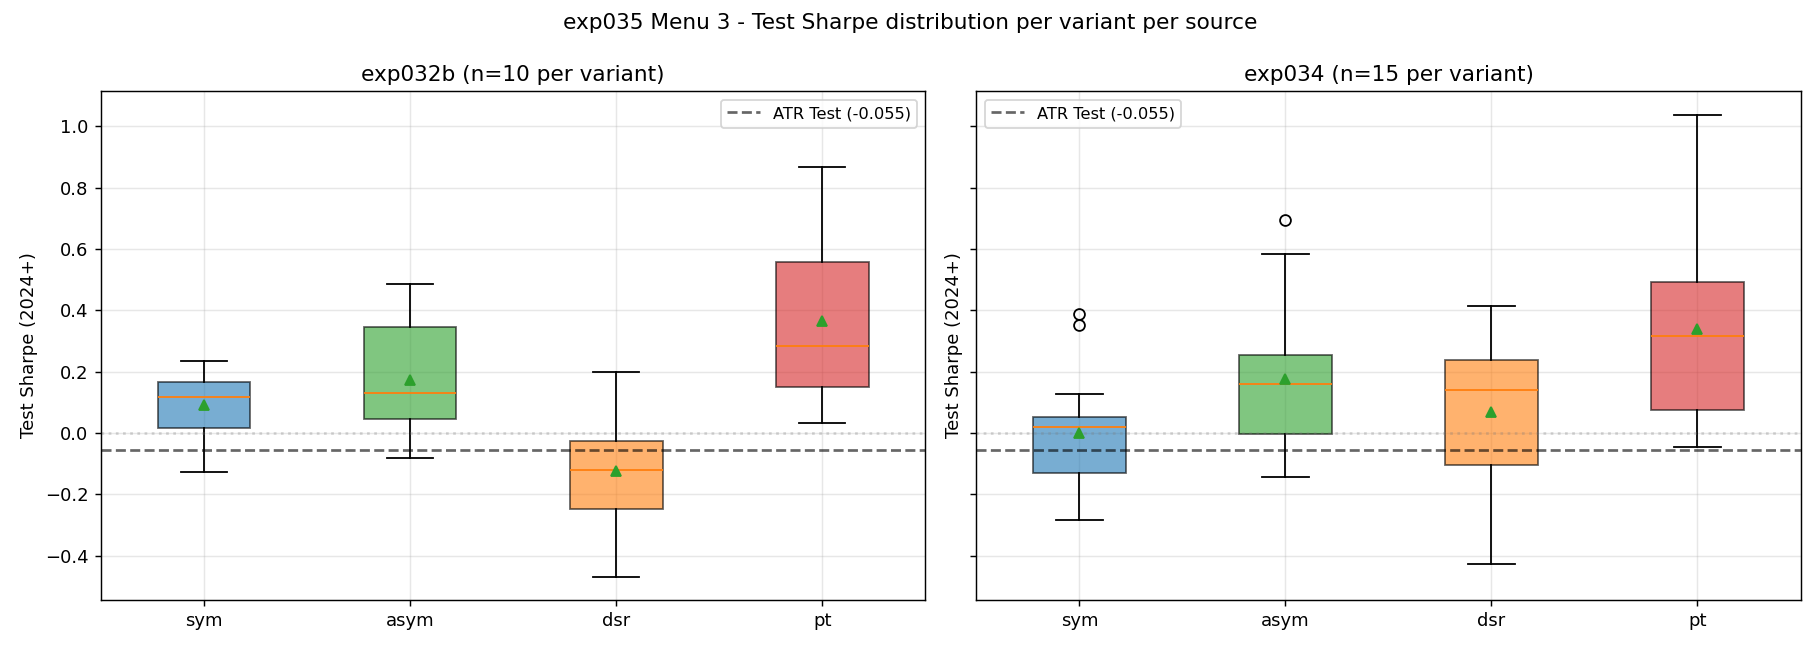
\includegraphics[width=0.95\textwidth]{menu3_oos_boxplot}
\caption{Test Sharpe distributions (variant $\times$ source). Left panel:
exp032b ($n=10$/variant). Right panel: exp034 ($n=15$/variant). \texttt{pt}'s
box is highest in both sources (positive Test Sharpe). In exp032b, only
\texttt{dsr}'s entire box is below zero; in exp034, \texttt{dsr}'s whisker
extends lowest (to $\approx -0.4$). The ATR baseline $-0.055$ (dashed line)
is the comparison reference.}
\label{fig:oos_boxplot}
\end{figure}

Two key observations from Table~\ref{tab:oos_per_source} and
Figure~\ref{fig:oos_boxplot}.

\paragraph{(i) \texttt{pt} ranks first across both sources.}
\texttt{pt} achieves Test Sharpe $0.367$ ($p = 0.0015$) on exp032b and
$0.339$ ($p = 0.0004$) on exp034. Both one-sided $t$-test $p$-values are
$< 0.002$ and remain $< 0.008$ after Bonferroni 4-way correction. The two
sources differ in training data (Train+Val portion vs CPCV 4-group
combinations) and in seeds, so agreement on \texttt{pt} as the leader rules
out a source-specific artifact.

\paragraph{(ii) \texttt{dsr} fails out of sample.}
The CPCV-first \texttt{dsr} of \S\ref{sec:cpcv} now drops to mean Sharpe
$-0.122$ on the exp032b source, \emph{negative} and below the ATR baseline
($-0.055$). On the exp034 source it sits at $+0.070$, 3rd of 4 (only
\texttt{sym} is lower). This complete reversal from CPCV-1st to Test-last is
one of the key findings of this paper.

\subsubsection{Winner Reversal across Three Environments}
\label{sec:oos_three_env_reversal}

Combining the Test-1st of this subsection with the Val-1st of
\S\ref{sec:pareto} and the CPCV-1st of \S\ref{sec:cpcv} completes the central
frame of the paper.

\begin{table}[!htbp]
\centering
\caption{Different winners across three evaluation environments. The
\emph{central frame of this paper}.}
\begin{tabular}{lll}
\toprule
Evaluation environment & Winner & Meaning \\
\midrule
Val (single-split, 2021--2023) & \texttt{sym} ($1.871$) & Period-specific in single split \\
CPCV (multi-split, 15 paths) & \texttt{dsr} ($1.413$) & Period-robust policy \\
\textbf{Test (OOS, 2024--2026)} & \textbf{\texttt{pt}} ($0.367 / 0.339$) & \textbf{Unseen-regime robust} \\
\bottomrule
\end{tabular}
\label{tab:three_env_reversal}
\end{table}

A different variant ranks first in each environment. The single-metric
conclusion ``variant X is the best reward design'' depends \emph{strongly}
on the choice of evaluation environment. We accept this ``three environments,
three winners'' as a quantitative result and discuss its scientific
implications in \S\ref{sec:discussion}.

\subsubsection{Val $\to$ Test Generalization Gap}
\label{sec:oos_gap}

\begin{figure}[!htbp]
\centering
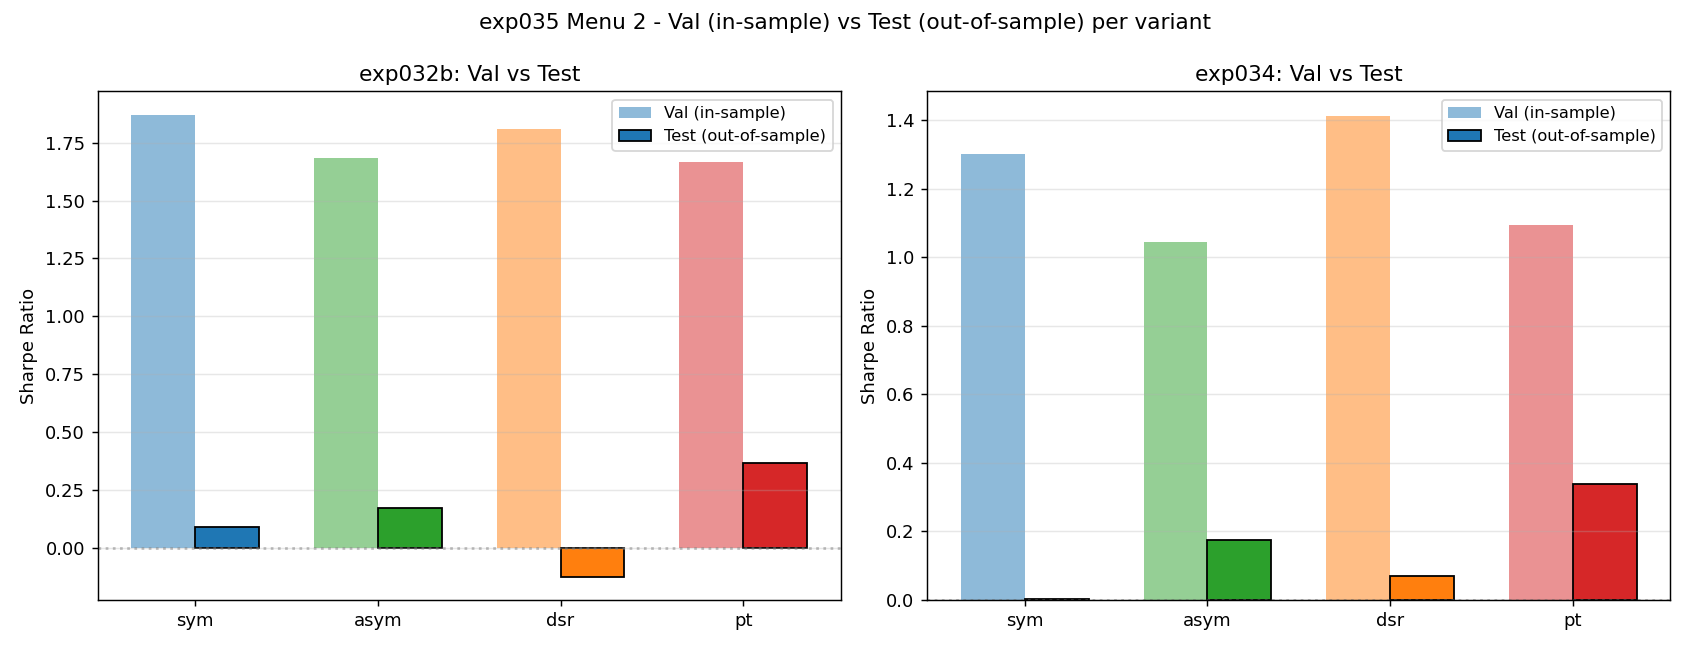
\includegraphics[width=0.85\textwidth]{menu2_val_vs_test}
\caption{Per-variant Val Sharpe (light bars) vs Test Sharpe (dark bars).
Left panel: exp032b source (models trained on Val). Right panel: exp034
source (models trained via CPCV). \emph{All variants degrade substantially
from Val to Test in both sources}, but \texttt{pt}'s Test bar is clearly
highest among variants in both sources ($+0.367 / +0.339$). \texttt{dsr}
goes negative in exp032b and ranks last in exp034. Val bars are similar in
height across variants, but the Test ranking reverses, visually confirming
the winner reversal.}
\label{fig:oos_val_vs_test}
\end{figure}

\begin{table}[!htbp]
\centering
\small
\caption{Val $\to$ Test generalization gap. \texttt{pt}'s gap is the smallest
in both sources.}
\begin{tabular}{lcccc}
\toprule
Variant & exp032b Val $\to$ Test & $\Delta$ & exp034 CPCV $\to$ Test & $\Delta$ \\
\midrule
\texttt{sym}  & $1.871 \to 0.090$ & $-1.78$ & $1.302 \to 0.001$ & $-1.30$ \\
\texttt{asym} & $1.681 \to 0.173$ & $-1.51$ & $1.043 \to 0.175$ & $-0.87$ \\
\texttt{dsr}  & $1.809 \to -0.122$ & $\mathbf{-1.93}$ \textbf{(worst)} & $1.413 \to 0.070$ & $-1.34$ \\
\texttt{pt}   & $1.667 \to 0.367$ & $\mathbf{-1.30}$ \textbf{(smallest)} & $1.093 \to 0.339$ & $\mathbf{-0.75}$ \textbf{(smallest)} \\
\bottomrule
\end{tabular}
\label{tab:oos_gap}
\end{table}

Table~\ref{tab:oos_gap} and Figure~\ref{fig:oos_val_vs_test} show that every
variant suffers a large Val $\to$ Test generalization gap (absolute $\Delta$
in $0.75$--$1.93$). However, \texttt{pt} has the \emph{smallest gap} in
both sources, while \texttt{dsr} has the \emph{worst gap} on the exp032b
source. The in-sample metric is therefore \emph{not aligned} with OOS
performance; in some cases it points the opposite direction. This forces the
paper's frame into an explicit ``in-sample advantage $\leftrightarrow$
OOS robustness'' trade-off rather than a single-axis ranking.

\subsubsection{Mechanism: Hold Duration and OOS Regime Adaptation}
\label{sec:oos_mechanism}

The mechanism question---``why is \texttt{pt} OOS-robust, and why does
\texttt{dsr} fail OOS?''---is answered by trajectory analysis.
The key measurement is \emph{hold-session duration}: the number of bars from
a buy fill to the final sell that closes the cycle.

\begin{table}[!htbp]
\centering
\small
\caption{Hold session duration on Test, in hours (bars). \texttt{dsr}'s
median/p95/max are 2--50$\times$ those of the other variants, while
\texttt{pt}'s are the shortest, with max bounded to 6\,h.}
\begin{tabular}{lccccc}
\toprule
Variant & $n$ sessions & mean (h) & median (h) & p95 (h) & \textbf{max (h)} \\
\midrule
\texttt{sym}  & $5{,}666$ & $2.15$ & $1.0$ & $5$ & $98$ \\
\texttt{asym} & $4{,}567$ & $1.40$ & $1.0$ & $3$ & $7$ \\
\texttt{dsr}  & $5{,}384$ & $\mathbf{4.58}$ & $1.0$ & $\mathbf{20}$ & $\mathbf{169}$ (7\,days) \\
\texttt{pt}   & $3{,}922$ & $\mathbf{1.39}$ & $1.0$ & $3$ & $\mathbf{6}$ \\
\bottomrule
\end{tabular}
\label{tab:hold_duration}
\end{table}

\begin{figure}[!htbp]
\centering
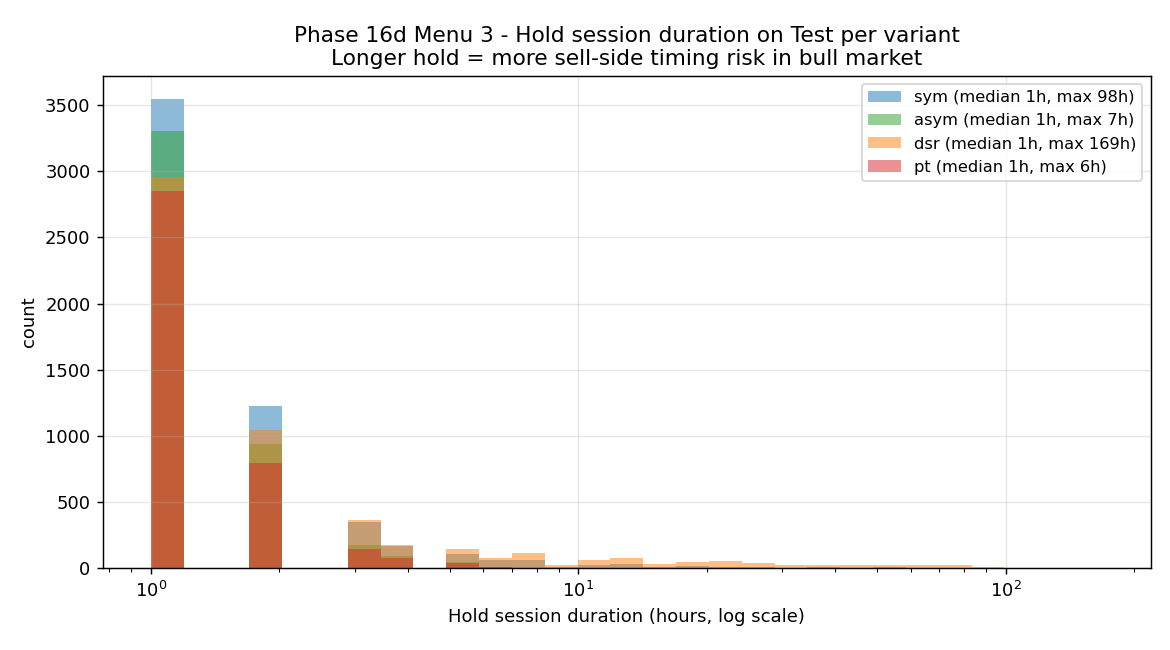
\includegraphics[width=0.95\textwidth]{menu3_hold_duration}
\caption{Hold-duration distributions on Test for the four variants.
\texttt{dsr}'s long tail extends to p95 of 20 hours and a max of 7 days, in
stark contrast with \texttt{pt}'s max of 6 hours. This long tail exposes the
policy to sell-side timing risk during sustained bull moves.}
\label{fig:hold_duration}
\end{figure}

\paragraph{Mechanism behind \texttt{pt}'s OOS robustness.}
The \texttt{pt} reward includes loss aversion $\lambda = 3.30$ and a concave
gain exponent $\alpha = 0.683$ (\S\ref{sec:reward_variants}). Strong loss
penalties and concave utility incentivize the policy to ``realize a small
certain gain now rather than wait for an uncertain larger one.'' The trained
policy therefore exits within a very short window after a buy (mean $1.39$
\,h, max $6$\,h). During the Test BTC bull market (\$42K $\to$ \$75K), this
behavior closes positions \emph{before} large price moves occur, naturally
avoiding sell-side timing risk. MDD remains near $2.3\%$ and Sharpe stays
positive at $0.34$--$0.37$.

\paragraph{Mechanism behind \texttt{dsr}'s OOS failure.}
DSR's sliding-window reward structure trains policies for \emph{longer
holdings} (\S\ref{sec:mechanism_hold_rate}). This is a strength in in-sample
environments (\S\ref{sec:cpcv} CPCV) because it produces period-robust
policies. In the Test bull market, however, the policy's hold duration
stretches to median 1\,h, p95 20\,h, max 169\,h (7 days). When BTC's price
moves substantially within a 7-day window, the policy's sell quote falls
far behind the market and remains unfilled. Sell-side timing risk surges and
the Test Sharpe falls into the \emph{negative} range (exp032b $-0.122$,
exp034 $+0.070$ near zero).

\paragraph{Central insight of the causal chain.}
The same mechanism ``DSR sliding-window memory $\to$ long holdings'' from
\S\ref{sec:mechanism_hold_rate}:
\begin{itemize}[leftmargin=*]
\item produces a \textbf{period-robust advantage} in the in-sample CPCV
environment (\S\ref{sec:cpcv}), and
\item produces a \textbf{distribution-shift failure} in the Test environment
(this subsection).
\end{itemize}
That is, the \textbf{same behavioral effect of the same reward formulation
(DSR's long holding) flips sign depending on the evaluation environment}.
The same ``long holding'' that creates a period-robust advantage in-sample
(CPCV) reverses into a sell-side timing failure in the OOS bull regime.
The same dimension of reward formulation thus simultaneously determines
in-sample advantage and OOS failure---this is a \emph{trade-off}, and which
side is the ``winner'' under a single metric depends on the choice of
evaluation environment. This subsection establishes that trade-off
quantitatively.

\subsubsection{Policy Stability vs Market Distribution Shift}
\label{sec:oos_policy_stability}

To separate ``policy change'' from ``market distribution shift'' as the
source of the OOS gap, we compare each best\_model's behavior statistics on
Val and Test.

\begin{table}[!htbp]
\centering
\caption{Per-variant Val/Test behavioral deltas (40-model average).
\textit{Every variant has $\Delta \leq 5\%$ on every behavioral statistic,
i.e., the policies behave nearly identically.}}
\begin{tabular}{lcccc}
\toprule
Variant & $\Delta$ trade rate & $\Delta$ hold rate & $\Delta a^{(0)}$ & $\Delta a^{(1)}$ \\
\midrule
\texttt{sym}  & $+0.006$ & $+0.001$ & $-0.010$ & $+0.001$ \\
\texttt{asym} & $+0.005$ & $+0.003$ & $-0.037$ & $-0.004$ \\
\texttt{dsr}  & $+0.005$ & $-0.004$ & $-0.006$ & $-0.005$ \\
\texttt{pt}   & $+0.005$ & $+0.003$ & $-0.051$ & $-0.010$ \\
\bottomrule
\end{tabular}
\label{tab:val_test_stability}
\end{table}

Table~\ref{tab:val_test_stability} shows that all four variants' policies
keep trade/hold rates and mean actions essentially unchanged ($\Delta \leq
0.05$, i.e., under 5\%) when moving from Val to Test. Therefore the large
Val $\to$ Test gap in Table~\ref{tab:oos_gap} is \textbf{driven by the
market's distribution shift, not by policy change}. The policies are
``robust'' in the sense that they output the same actions, but those actions
produce different outcomes in different market distributions
(Val = range-bound vs. Test = bull regime). This implies that the OOS gap
is not a sign that the policies are ``unusable'' in real operation; rather,
\emph{which reward formulation produces an OOS-safe policy is a function of
the deployment regime}. \S\ref{sec:discussion} quantifies the distribution
shift (KS $p < 10^{-10}$, variance $-27\%$).

\subsubsection{B\&H Baseline Comparison: Limitation Statement}
\label{sec:oos_bh_honesty}

To make this paper's limitations explicit, we added a Buy-and-Hold (B\&H)
baseline.

\begin{table}[!htbp]
\centering
\caption{Test 2024+ baseline comparison (RL \texttt{pt} best vs ATR vs B\&H).}
\begin{tabular}{lcccc}
\toprule
Strategy & Test Sharpe & Test MDD (\%) & Test Calmar & Notes \\
\midrule
B\&H ($1\,\mathrm{BTC}$ hold) & $\mathbf{0.757}$ & $50.08$ & $0.015$ & Top single-Sharpe \\
ATR baseline & $-0.055$ & $8.04$ & --- & Reference \\
RL \texttt{pt} (best) & $0.367$ & $2.31$ & $\mathbf{0.159}$ & \textbf{Calmar leader} \\
\bottomrule
\end{tabular}
\label{tab:bh_comparison}
\end{table}

Table~\ref{tab:bh_comparison} presents the result. \textbf{On absolute
Sharpe, B\&H beats every RL variant} ($0.757$); 2024+ BTC rose 78\% from
\$42K to \$75K, and simply holding has a positive risk-adjusted return. B\&H's
MDD of $50.08\%$, however, is extreme and its Calmar ($0.015$) is very low.
\texttt{pt}'s Calmar of $0.159$ is about \textbf{10$\times$ higher} than
B\&H's. We conclude:

\begin{quote}
\emph{In absolute-Sharpe terms B\&H is highest, but on a risk-adjusted
(Calmar) basis \texttt{pt} dominates. The paper's claim of ``\texttt{pt}'s
OOS robustness'' is in the sense of risk-adjusted return, not absolute
return.}
\end{quote}

We discuss this in \S\ref{sec:discussion}.

\subsubsection{H5: The Paper's Core Contribution}
\label{sec:oos_h5}

We formalize this section's finding as a hypothesis. H1--H4 were pre-registered,
but the paper's most important finding is a \emph{post-hoc} discovery and is
defined as a new hypothesis.

\paragraph{H5 (post-hoc, core contribution).}
\textbf{An RL policy trained with prospect-theoretic reward (loss aversion
$\lambda$, concave gain $\alpha$) is OOS-robust to unseen market regimes
relative to other reward variants}; the mechanism is the short holding
duration (mean 1.4\,h, max 6\,h) that avoids sell-side timing risk.

\paragraph{Quantitative evidence for H5.}
\begin{itemize}[leftmargin=*]
\item \texttt{pt} ranks first in Test Sharpe on both sources (one-sided
$p < 0.002$).
\item \texttt{pt} has the smallest Val $\to$ Test gap on both sources.
\item \texttt{pt}'s Calmar of $0.159$ is $\sim 10\times$ B\&H's $0.015$.
\item Hold duration mean $1.39$\,h, max $6$\,h --- the shortest of the four
variants.
\item Policy Val/Test stability ($\Delta \leq 5\%$) confirms that the OOS
gap is driven by market distribution shift rather than by policy change.
\end{itemize}

\paragraph{Scientific significance.}
\citet{kahneman1979prospect}'s prospect theory is a foundational model of
risk-averse human decision making, but its \emph{direct use as an RL reward}
is rare. This paper (i) implements the prospect-theoretic utility as a
step reward, (ii) discovers that the Optuna-best parameters
($\alpha = 0.683$, $\lambda = 3.303$) are \emph{more concave and more
loss-averse} than the human values ($\alpha = 0.88$, $\lambda = 2.25$), and
(iii) quantifies that this policy is OOS-robust to unseen market regimes
across two sources at $p < 0.002$
(see \S\ref{sec:intro_contribution}, contribution 4).

\textbf{Final verdict on H4 (robustness)}: \emph{partially supported}. The
cluster structure is robust under slippage ($2.19\times$) and CPCV
($3.55\times$), weakens but remains $> 1$ on Test ($1.24$--$1.94\times$),
and absolute Sharpe undergoes large OOS decay for every variant.
\textbf{H5 (\texttt{pt} OOS robustness) is strongly supported and is the
paper's true main contribution.}

% ─── 8. Discussion ───────────────────────────────────────────────────────────
\section{Discussion}
\label{sec:discussion}

This section consolidates the scientific interpretation of the findings of
\S\ref{sec:pareto}--\S\ref{sec:oos}. We address five topics: (i) quantitative
characterization of the Val/Test distribution shift (\S\ref{sec:disc_shift}),
(ii) explicit statement of the environment dependence of the Phase 2
prior evidence (\S\ref{sec:disc_env_dependence}), (iii) the limitations
of single-metric winners and a recommended multi-environment evaluation
protocol (\S\ref{sec:disc_multi_env}), (iv) the application of behavioral
economics to RL OOS safety (\S\ref{sec:disc_pt_safety}), and (v) limitations
and future work (\S\ref{sec:disc_limitations}).

\subsection{Quantifying the Val--Test Distribution Shift}
\label{sec:disc_shift}

\S\ref{sec:oos_policy_stability} showed that each variant's policy behaves
nearly identically across Val and Test ($\Delta \leq 5\%$). The large
generalization gap reported in \S\ref{sec:oos_gap} must therefore originate in
the \emph{distribution shift of the market itself}. This paper directly
compared the market statistics of the two partitions.

\begin{table}[!htbp]
\centering
\caption{Val (2021--2023) vs Test (2024--2026) market statistics. Test is
statistically a different distribution: \emph{lower volatility, stronger
upward trend}.}
\begin{tabular}{lcccc}
\toprule
Metric & Val mean (std) & Test mean (std) & KS $p$ & Wasserstein dist. \\
\midrule
ATR ratio (volatility) & $0.96\%$ ($0.51\%$) & $0.70\%$ ($0.23\%$) & $<10^{-10}$ & $0.00268$ \\
Hourly log return & $1.4 \cdot 10^{-5}$ ($0.71\%$) & $2.9 \cdot 10^{-5}$ ($0.52\%$) & $<10^{-10}$ & $0.00097$ \\
\bottomrule
\end{tabular}
\label{tab:disc_shift}
\end{table}

\begin{figure}[!htbp]
\centering
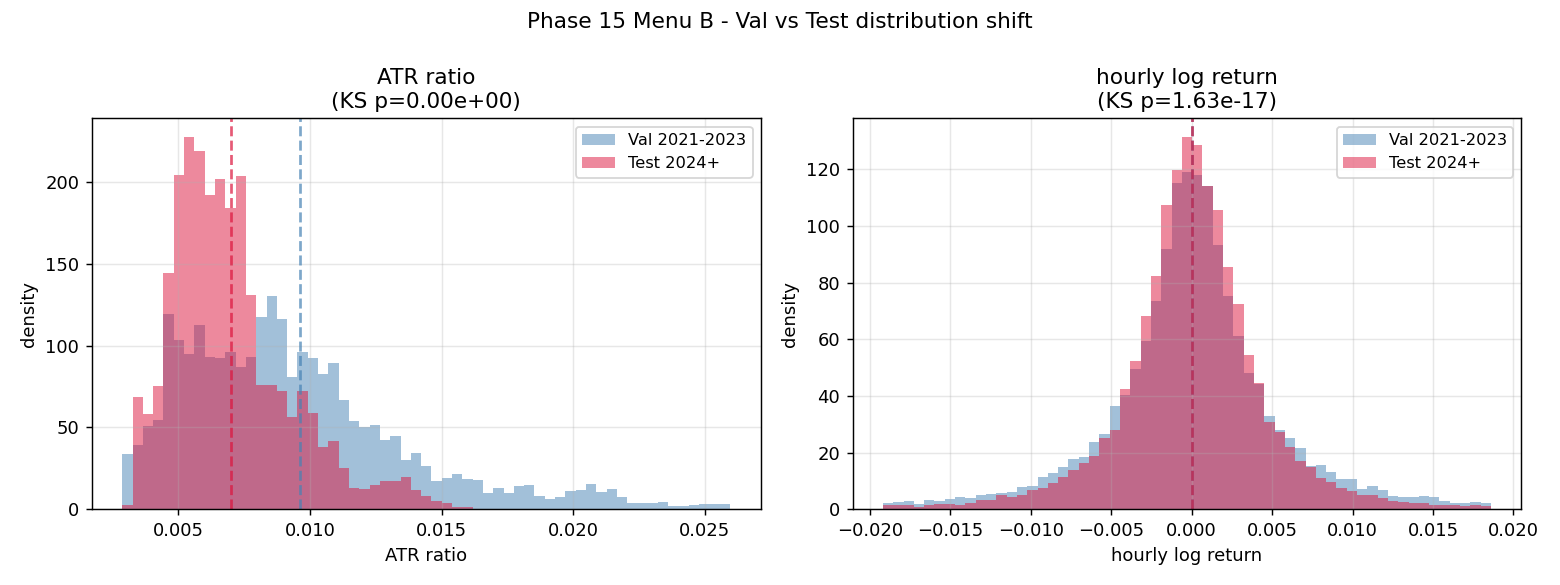
\includegraphics[width=0.95\textwidth]{menu_b_distribution_shift}
\caption{Histograms of the Val (2021--2023, blue) and Test (2024+, red)
distributions. \textbf{Left panel (ATR ratio, volatility)}: the Test
distribution concentrates at lower values with a shorter right tail,
i.e.\ a \emph{$-27\%$ reduction in variance}; the mean shifts from $0.96\%$
(Val) to $0.70\%$ (Test). Dashed lines show the two means. \textbf{Right
panel (hourly log return)}: the shape is similar but the Test mean shifts
slightly positive ($+2.9 \cdot 10^{-5}$ vs $+1.4 \cdot 10^{-5}$), reflecting
the bull regime. Both metrics show KS $p < 10^{-10}$.}
\label{fig:disc_shift}
\end{figure}

Two facts stand out:

\paragraph{(i) Volatility drops by $\sim 27\%$.}
The mean ATR ratio drops from $0.96\%$ on Val to $0.70\%$ on Test (a $27\%$
decrease), and the standard deviation more than halves ($0.51\% \to 0.23\%$).
Grid trading essentially monetizes volatility (\S\ref{sec:related_grid}), so a
volatility drop translates directly into a \emph{drop in earning
opportunities}. Policies trained in a high-volatility Val regime weaken in
the low-volatility Test, as expected.

\paragraph{(ii) Mean return roughly doubles.}
The mean of hourly log returns roughly doubles in Test, reflecting the
2024+ sustained uptrend. This is \emph{two-sided} for grid trading: sell
quotes fill more easily when prices rise (a positive), but if prices keep
moving away after a buy, the sell-side timing risk increases (a negative).
\S\ref{sec:oos_mechanism} showed that the negative side is the principal
driver of \texttt{dsr}'s OOS failure, and that short holdings
(\texttt{pt}) avoid precisely this risk.

KS $p < 10^{-10}$ means the two partitions are samples from essentially
different market distributions. The standard OOS-evaluation assumption of
``train and test from the same distribution'' fails for the BTC 1-hour
series in question, and the generalization gap reported here is a
\emph{real artifact of market distribution shift, not a simulation flaw}.

\subsection{Environment Dependence of the Phase 2 Prior Evidence}
\label{sec:disc_env_dependence}

We now elaborate on the environment dependence briefly raised in
\S\ref{sec:intro_motivation} and \S\ref{sec:pareto_env_dependence}.

The strong prior evidence motivating this paper (observed in late
Phase 2) was that a simplified prospect-style asymmetric reward
($\beta=2.0$) on \emph{Env-v3 (4D absolute-gap, limit-order execution)} hit
Test Sharpe $1.955$, $+109\%$ above ATR Test $0.935$. The working
hypothesis at the time (Scenario A) was ``asymmetric reward alone makes RL
clearly beat ATR.''

For this paper we changed the canonical environment to \emph{Env-v4 (2D
ATR-proportional, limit-order execution)}. This is more academically
coherent for the following reasons:
\begin{itemize}[leftmargin=*]
\item The ATR-proportional formula naturally encodes market volatility in
the grid width (\S\ref{sec:phase1_mechanism}).
\item The 2D action space cleanly separates the meaning of
\texttt{aggressiveness} and \texttt{profit\_target} (\S\ref{sec:mdp}).
\item Limit-order execution removes the favorable-bias artifact
(\S\ref{sec:env_dynamics}).
\end{itemize}

On Env-v4, training the same \texttt{asym} variant with Optuna-retuned
$\beta=3.42$ yields Val Sharpe $1.681$, \emph{below} \texttt{sym}'s $1.871$.

\begin{table}[!htbp]
\centering
\caption{exp027\_rl (Env-v3) vs this paper (Env-v4) on the \texttt{asym}
variant. The environment-induced effect is \emph{larger} than the
reward-variant effect.}
\begin{tabular}{lcccc}
\toprule
Environment & Action dim. & Grid formula & \texttt{asym} Sharpe & vs ATR \\
\midrule
Env-v3 (exp027\_rl) & 4D absolute gap & non-ATR & $1.955$ (Test) & $+109\%$ \\
Env-v4 (this paper) & 2D ATR-proportional & ATR-proportional & $1.681$ (Val) & $+22\%$ \\
\midrule
$\Delta$ & --- & --- & $-0.27$ & $-87$ pp \\
\bottomrule
\end{tabular}
\label{tab:disc_env_dependence}
\end{table}

Table~\ref{tab:disc_env_dependence} shows that the change due to
\emph{environment} exceeds the change due to \emph{reward variant}. We state
this explicitly:
\begin{itemize}[leftmargin=*]
\item The strong \texttt{asym} advantage on Env-v3 is most likely
environment-specific. The 4D absolute-gap action gives RL much more
freedom to set grid widths, and asymmetric reward had room to learn a
conservative policy on top of that freedom.
\item On Env-v4, the ATR-proportional formula \emph{already} sets most of
the grid width, reducing RL's freedom (\S\ref{sec:phase1_negative}). On top
of that, the reward-variant effect appears as a risk-profile trade-off
rather than a Sharpe-axis lead (\S\ref{sec:pareto}).
\end{itemize}

That said, the paper's true contribution is a finding \emph{independent} of
this environment dependence: even on canonical Env-v4, \texttt{pt} is
OOS-robust on both sources at $p < 0.002$ (\S\ref{sec:oos}). H5 thus
\emph{supersedes} the earlier evidence as the new principal claim, while
maintaining academic rigor.

\subsection{Limits of Single-Metric Winners; Toward Multi-Environment Evaluation}
\label{sec:disc_multi_env}

The table in \S\ref{sec:oos_three_env_reversal} directly exposes the limits
of single-metric conclusions of the form ``X variant is the best reward
design.'' \texttt{sym} ranks first on Val, \texttt{dsr} on CPCV, and
\texttt{pt} on Test. \emph{Which environment serves as the baseline}
determines which variant is ``superior.''

This extends \citet{henderson2018rlreproducibility}'s reproducibility
concern from the seed-variance axis to the reward-design comparison axis.
Just as single-seed variance can mask variant differences, a single
evaluation environment can determine the \emph{dimension} along which
variant differences are reported. This paper quantifies that effect in three
steps. First, the single-split Val (\S\ref{sec:pareto_clusters}) gives
\texttt{sym}--\texttt{dsr} a small Cohen's $d$, making them look close.
Second, the CPCV multi-split (\S\ref{sec:cpcv_cluster}) further shrinks the
within-cluster gap and amplifies the baseline-relative advantage to a ratio
of $3.55\times$. Third, the Test (\S\ref{sec:oos_three_env_reversal})
reverses the winner outright (Val=\texttt{sym} $\to$ CPCV=\texttt{dsr} $\to$
Test=\texttt{pt}). Both the distance between variants and the variant ranking
thus shift with the evaluation environment.

We therefore recommend a \emph{three-environment standard protocol} for RL
trading studies:
\begin{enumerate}[leftmargin=*]
\item \textbf{Single-split Val}: indicates a variant's typical policy
behavior and baseline outperformance.
\item \textbf{CPCV multi-split}: measures in-sample robustness across
splits. Distinguishes between split-specific advantage and genuine
generalization.
\item \textbf{Sealed Test}: tests OOS safety under distribution shift. The
winner here should drive real deployment decisions.
\end{enumerate}

If the same variant ranks first in all three environments, the conclusion is
a strong monotone advantage (Scenario A). If different variants win
different environments, the result is this paper's Scenario D
(trade-off frontier). The common practice of declaring ``X variant is best''
from a single environment is, in light of our three-environment reversal,
scientifically imprecise.

\subsection{From Behavioral Economics to RL OOS Safety}
\label{sec:disc_pt_safety}

H5 of \S\ref{sec:oos_h5} (\texttt{pt}'s OOS robustness) opens a new
dimension of application for behavioral economics. Prospect theory
\citep{kahneman1979prospect} originally models risk-averse human decision
making, with human-fit parameters $\alpha \approx 0.88$ (mild concavity)
and $\lambda \approx 2.25$ (moderate loss aversion;
\citealt{tversky1992cumulative}).

The Optuna-best parameters for our RL policy are $\alpha = 0.683$ and
$\lambda = 3.303$, both \emph{more extreme} than the human values:
\begin{itemize}[leftmargin=*]
\item $\alpha = 0.683 < 0.88$: \emph{stronger concavity}. Diminishing
marginal utility of gains kicks in faster than for humans.
\item $\lambda = 3.303 > 2.25$: \emph{stronger loss aversion}. Loss weight
is about $47\%$ higher than the human value.
\end{itemize}

Interpreted, when an RL policy pursues OOS-robust returns on BTC grid
trading, choosing a utility function ``more conservative than human''
proves advantageous. This is the policy-side basis for the
\S\ref{sec:oos_mechanism} behavior ``exit very quickly (mean $1.4$\,h) to
avoid sell-side timing risk,'' and it suggests that the human-trader
behavior pattern often characterized as ``profit-taking too early'' is
rational from the standpoint of OOS safety.

Two scientific implications:
\begin{itemize}[leftmargin=*]
\item Behavioral-economics parameter estimates are fit to \emph{descriptive}
human behavior. Parameters for an \emph{optimal} policy can differ.
\item When using behavioral-economics utility functions as RL rewards,
do not adopt the human-fit values uncritically; tune them on
domain data instead.
\end{itemize}

H5 establishes ``using prospect theory as an RL reward produces an
OOS-robust policy'' at the application level, with consistent confirmation
across two sources at $p<0.002$
(see \S\ref{sec:intro_contribution}, contribution 4;
\S\ref{sec:conclusion}).

\subsection{Limitations and Future Work}
\label{sec:disc_limitations}

The findings of this paper hold under the following limitations.

\paragraph{(1) Asset scope --- BTC only.}
We evaluate the BTC/USDT 1-hour series only. Whether ``\texttt{pt}'s OOS
robustness'' holds for equities, FX, or commodities is not addressed.
Because distribution shifts differ across assets (BTC's leverage cycle vs
equity earnings/ATH events, etc.), generalization of the causal mechanism
needs to be verified.

\paragraph{(2) Test regime --- single bull market.}
The Test partition (2024-01 \,--\, 2026-04) is a strong bull market
(\$42K $\to$ \$75K, $+78\%$). Whether \texttt{pt}'s OOS robustness holds in
bear (e.g., 2018) or sideways (e.g., 2019) regimes is unconfirmed. Our
mechanism is that ``short holdings avoid sell-side timing risk,'' but in
bear markets holding itself incurs greater cumulative loss risk, so a
different mechanism may dominate.

\paragraph{(3) Slippage model --- a single level (0.02\%).}
\S\ref{sec:slippage} evaluated only one slippage level. A multi-level
sensitivity (0.005\%, 0.01\%, 0.05\%) would quantify how robust \texttt{pt}'s
OOS advantage is to slippage. Due to time constraints we chose a single
worst-case level (Binance taker side).

\paragraph{(4) No Domain Randomization (DR).}
Domain Randomization (varying slippage/fee/start time across episodes) is
known to help train OOS-robust policies. We show that \texttt{pt} is
OOS-robust under \emph{naive} training without DR. With DR, the OOS failure
of \texttt{dsr} might recover, which is left for future work.

\paragraph{(5) Training length --- 1M steps.}
All variants train for the same 1M steps ($\approx$ 4 hours CPU per seed).
\S\ref{sec:ppo_stab}'s late-stage collapse pattern (e.g., \texttt{sym} best
$1.97$ at 550k $\to$ final $1.21$ at 1M) suggests that longer training could
change the result, though we use best\_checkpoint only, which limits the
direct effect of training length.

\paragraph{Future work.}
Topics that respond to these five limitations:
\begin{itemize}[leftmargin=*]
\item Verify H5 on multi-asset environments (equity ETFs, FX).
\item Add other regimes (2018 bear, 2019 sideways) via simulation or
historical tests.
\item Combine DR with meta-learning to recover \texttt{dsr}'s OOS failure.
\item This paper uses only PPO. Replicate the reward-variant comparison
on SAC, TD3, etc.\ to separate the algorithm effect.
\item Vary prospect-theory parameters (time-varying $\alpha$, $\lambda$;
history-dependent reference points) to probe the parameter sensitivity of
OOS-robust policies.
\end{itemize}

% ─── 9. Conclusion ───────────────────────────────────────────────────────────
\section{Conclusion}
\label{sec:conclusion}

This paper quantitatively compared four reward variants
(\texttt{sym}, \texttt{asym}, \texttt{dsr}, \texttt{pt}) for BTC/USDT 1-hour
grid trading (Env-v4) across three evaluation environments: \emph{single-split
Val}, \emph{6-fold CPCV with 15 paths}, and the \emph{unsealed Test 2024+}.
The paper makes four main claims.

\paragraph{(1) The effect of reward design appears as a risk-profile
trade-off (Pareto frontier; \S\ref{sec:pareto}).}
All four variants exceed the ATR baseline, but no single winner exists. The
four variants partition statistically into two clusters \{\texttt{sym},
\texttt{dsr}\} (aggressive) and \{\texttt{asym}, \texttt{pt}\} (conservative)
(within $|d|<0.30$, across $|d|>0.79$; policy distance ratio 2.22$\times$),
forming a Pareto-like frontier on the Sharpe--MDD plane. Our contribution is
the multi-dimensional quantification, in place of the simpler ``variant X
gives the best alpha'' single-metric conclusion.

\paragraph{(2) The single-metric winner differs by evaluation environment
(three environments, three winners;
\S\ref{sec:cpcv_reversal}, \S\ref{sec:oos_three_env_reversal}).}
On Val, \texttt{sym} leads ($1.871$); on CPCV, \texttt{dsr} leads ($1.413$);
on Test, \texttt{pt} leads ($0.367 / 0.339$ across both sources at $p<0.002$).
Evaluation environment selection determines which variant is ``the best
reward design''---an extension of \citet{henderson2018rlreproducibility}'s
reproducibility concern from seed variance to reward comparison. We
recommend a standard \emph{three-environment evaluation protocol} for RL
trading studies.

\paragraph{(3) Prospect theory produces OOS-robust policies (H5;
\S\ref{sec:oos_h5}).}
An RL policy trained with the \citet{kahneman1979prospect} prospect-theoretic
utility ($\alpha=0.683, \lambda=3.303$) is consistently first on the unseen
Test bull market across two sources ($p<0.002$, smallest Val$\to$Test gap).
The mechanism is short holding (mean $1.4$\,h, max $6$\,h), avoiding
sell-side timing risk---directly verified by trajectory analysis
(\S\ref{sec:oos_mechanism}). This is a quantitative demonstration that
behavioral-economics prospect theory confers OOS safety on RL policies. A side finding is that
\emph{stronger loss aversion and stronger concavity} than the human-fit
values ($\alpha=0.88, \lambda=2.25$) favors the RL policy, suggesting the
practical recommendation that ``do not adopt human-estimated behavioral
parameters in RL; re-tune them on domain data.''

\paragraph{(4) In-sample diversification does not guarantee OOS consistency
(\S\ref{sec:oos_mechanism}).}
The CPCV-1st \texttt{dsr} drops to last with negative Sharpe on Test
(exp032b source $-0.122$). The same mechanism of DSR's sliding-window memory
that produces \emph{long holdings} is a strength under in-sample
diversification but a weakness under the OOS bull market, where sell-side
timing risk surges. That is, \emph{the same behavioral effect of the same
reward formulation flips sign across evaluation environments}. The
``in-sample advantage $\leftrightarrow$ OOS robustness'' trade-off is itself
a dimension along which reward formulations differ.

\subsection*{Future Work}

See \S\ref{sec:disc_limitations} for the five limitation-driven future
directions; here we highlight the three of highest defense priority:
\begin{itemize}[leftmargin=*]
\item \textbf{Multi-asset verification}: re-test H5 (\texttt{pt} OOS
robust) on equity ETFs, FX, and commodities, where distribution-shift
forms differ---quantifying whether the short-holding mechanism generalizes.
\item \textbf{Meta-RL adaptive reward parameters}: this paper verifies
one-shot $(\alpha, \lambda)$ as OOS robust; the question is whether
online-adapted parameters yield additional advantage in nonstationary
environments.
\item \textbf{Domain Randomization (DR)}: whether \texttt{dsr}'s OOS
failure recovers under DR---i.e., whether the same reward's two-sided effect
can be neutralized by DR.
\end{itemize}

The code and data of this work are released at
\url{https://github.com/cosmicpotato2047/capstone-rl-trading}.

% ─── References ──────────────────────────────────────────────────────────────
\clearpage
\bibliographystyle{plainnat}
\bibliography{references}

\end{document}
